\documentclass[12pt, a4paper]{report} % 'report' class is common for theses

% Use the custom style package
\usepackage{beekeepers_thesis_style}

% --- Document Information (for title page and PDF metadata) ---
\title{Розробка веб-платформи для комунікації та обміну знаннями в спільноті бджолярів}
\author{Едуард АНДРАЩУК}
\date{Київ — 2025}

% Graphics path (if images are in a subdirectory)
\graphicspath{{images/}}

\begin{document}

% --- Title Page ---
% --- Title Page Content ---
% This file will be input into the main thesis document.
% Customize with your specific university, department, student, and supervisor details.

\begin{titlepage}
    \centering
    \vspace*{1cm}
    % \universitylogo % Uncomment if you have a logo defined in the .sty file
    
    {\Large МІНІСТЕРСТВО ОСВІТИ І НАУКИ УКРАЇНИ\par}
    \vspace{0.5cm}
    {\Large Київський національний університет імені Тараса Шевченка\par}
    \vspace{0.5cm}
    {\Large Факультет комп'ютерних наук та кібернетики\par}
    \vspace{0.5cm}
    {\Large Кафедра математичної інформатики\par}
    
    \vfill % Pushes content to vertical center and bottom
    
    {\bfseries\Large МАГІСТЕРСЬКА РОБОТА\par}
    \vspace{0.5cm}
    {\Large на тему:\par}
    \vspace{1cm}
    {\bfseries\huge Розробка веб-платформи для комунікації та обміну знаннями в спільноті бджолярів\par}
    
    \vspace{2cm}
    
    {\Large зі спеціальності 122 "Комп'ютерні науки"\par}
    
    \vfill
    
    \begin{flushright}
    \vspace{1cm}
    {\Large Виконав:\par}
    {\Large Студент 2 курсу\par}
    {\Large Групи БІ-2\par}
    {\Large Едуард АНДРАЩУК\par}
    \vspace{0.5cm}
    {\Large \underline{\hspace{5cm}} (підпис)\par}
    \vspace{1cm}
    {\Large Науковий керівник:\par}
    {\Large доктор наук, професор\par}
    {\Large ВОЛОДИМИР Заславський\par}
    \vspace{0.5cm}
    {\Large \underline{\hspace{5cm}} (підпис)\par}
    \end{flushright}
    
    \vfill % Pushes the following content to the bottom
    
    {\Large Київ — 2025\par}
    \vspace*{1cm}
    
\end{titlepage}  % Include the title page content

\cleardoublepage
\pagenumbering{roman} % Roman numerals for front matter

% --- Abstract (Ukrainian) ---
% --- Abstract in Ukrainian ---
\begin{otherlanguage}{ukrainian}
\begin{abstract}
\noindent

Магістерська робота присвячена проектуванню та розробці повностекового веб-застосунку \textit{Beekeepers Community Platform} — інтегрованої платформи, призначеної для української спільноти бджолярів з метою сприяння ефективній комунікації, обміну спеціалізованими знаннями та надання інструментів для управління пасіками і полями.

У роботі здійснено аналіз предметної області, розглянуто існуючі рішення для нішевих онлайн-спільнот та інструменти для агросектору. Обґрунтовано вибір сучасного технологічного стеку, що включає React (з TypeScript, Vite, Material-UI, Redux Toolkit) для розробки клієнтської частини, NestJS (Node.js, Fastify, TypeScript) для серверної логіки, та MongoDB (з Mongoose) як документо-орієнтовану базу даних з підтримкою GeoJSON.

Спроектовано архітектуру платформи для комунікації та обміну знаннями в спільноті бджолярів, що базується на принципах модульності та RESTful API. Визначено функціональні та нефункціональні вимоги. Розроблено ключові модулі: система автентифікації користувачів (локальна реєстрація, верифікація email з можливістю повторного надсилання листа, Google OAuth, JWT для авторизації), форум для обговорень, структурована база знань, та багатофункціональна інтерактивна карта. Картографічний модуль дозволяє користувачам додавати, переглядати, редагувати метадані та видаляти об'єкти пасік (вулики) і полів, а також візуалізує попередження про заплановані обробки полів шляхом динамічного кольорового кодування.

Описано процес розробки, організацію кодової бази, ключові аспекти реалізації API та інтерфейсу користувача, включаючи використання Leaflet для картографії. Розглянуто питання безпеки, валідації даних та інтернаціоналізації.

Проведено тестування основних функціональних можливостей. За результатами роботи сформульовано висновки щодо успішної реалізації прототипу платформи та окреслено перспективні напрямки для її подальшого розвитку та вдосконалення.

\textbf{Ключові слова:} веб-застосунок, спільнота бджолярів, React, NestJS, MongoDB, інтерактивна карта, Leaflet, GeoJSON, управління пасіками, автентифікація, форум, база знань, RTK Query, Material-UI.
\end{abstract}
\end{otherlanguage} 
\cleardoublepage

% --- Abstract (English) ---
% --- Abstract in English ---
\begin{otherlanguage}{english}
\begin{abstract}
\noindent

This master's thesis focuses on the design and development of a full-stack web application named \textit{Beekeepers Community Platform} — an integrated platform designed for the Ukrainian beekeeping community to facilitate effective communication, specialized knowledge exchange, and provide tools for apiary and field management.

The work includes an analysis of the subject area, a review of existing solutions for communities, and a justification for the chosen technology stack, which includes React for the frontend, NestJS for the backend, and MongoDB as the database.

The platform architecture was designed, and functional and non-functional requirements were defined. Key modules have been developed, such as a forum for discussions, a knowledge base, an interactive map for managing apiaries and fields, and a user authentication mechanism with email verification and Google Sign-In capability.

The development process, code structure, API design principles, and main components of the beekeepers community platform are described. Security considerations were addressed, and appropriate mechanisms were implemented.

Testing of the main functional capabilities of the application was conducted. Based on the results, conclusions were formulated, and directions for further platform development were outlined.

\textbf{Keywords:} web application, beekeepers community, React, NestJS, MongoDB, forum, knowledge base, interactive map, authentication, OAuth.
\end{abstract}
\end{otherlanguage} 
\cleardoublepage

% --- Table of Contents ---
\tableofcontents
\cleardoublepage

% --- List of Figures (optional, if you have figures) ---
\listoffigures
\addcontentsline{toc}{chapter}{\listfigurename}
\cleardoublepage

% --- List of Tables (optional, if you have tables) ---
\listoftables
\addcontentsline{toc}{chapter}{\listtablename}
\cleardoublepage

% --- Introduction (Input before main content) ---
% --- Introduction ---
\chapter*{Вступ}
\addcontentsline{toc}{chapter}{Вступ}
\label{ch:introduction}

Актуальність теми магістерської роботи зумовлена зростаючою потребою у спеціалізованих онлайн-платформах для нішевих спільнот, зокрема для бджолярів, та визначається низкою ключових факторів. По-перше, бджільництво відіграє незамінну роль не лише як галузь сільського господарства, що забезпечує виробництво меду, воску, прополісу та інших цінних продуктів, але й як фундаментальний елемент підтримки біорізноманіття та екологічної стабільності через запилення ентомофільних культур та дикорослих рослин. За оцінками експертів, близько третини продовольства, що споживається людством, залежить від запилення комахами, серед яких бджоли є одними з найефективніших.

По-друге, сучасні бджолярі стикаються зі значними викликами, що загрожують як окремим пасікам, так і галузі в цілому. До таких викликів належать поширення хвороб та шкідників бджіл (наприклад, кліщ Варроа, американський гнилець), негативний вплив змін клімату на медоносні ресурси та життєдіяльність бджолосімей, а також масове використання пестицидів у сільському господарстві, що часто призводить до отруєння бджіл. В цих умовах оперативний обмін достовірною інформацією, передовим досвідом щодо профілактики та лікування хвороб, адаптації до кліматичних змін та безпечного співіснування з аграрним виробництвом набуває критичного значення.

По-третє, існуючі загальні соціальні мережі, месенджери та форуми, хоча й використовуються бджолярами для спілкування, не завжди враховують специфічні потреби та унікальний контекст бджолярської спільноти. Вони не надають спеціалізованих інструментів для обговорення вузькопрофільних тем, таких як ветеринарія бджіл, селекція, технології догляду за бджолосім\'ями, особливості медоносних рослин у конкретних регіонах. Особливо гострою є проблема координації дій щодо попередження отруєнь бджіл через обробку сільськогосподарських полів та ефективного планування розташування пасік з урахуванням кормової бази та санітарно-епідеміологічної ситуації.

Таким чином, розробка спеціалізованої веб-платформи, що інтегрує засоби комунікації, базу знань, інструменти для обміну оперативною інформацією (зокрема, про обробки полів) та можливості для ведення обліку пасік, є надзвичайно актуальним завданням. Така платформа може суттєво сприяти підвищенню ефективності бджільництва, збереженню бджолосімей, покращенню координації між пасічниками та іншими зацікавленими сторонами, а також слугувати інструментом для збору та аналізу даних, важливих для розвитку галузі та моніторингу екологічного стану.

Метою даної магістерської роботи є розробка фулстек веб-застосунку \textit{Beekeepers Community Platform}, що надасть бджолярам зручні інструменти для комунікації, обміну інформацією, доступу до бази знань та управління даними про власні пасіки та сільськогосподарські угіддя.

Для досягнення поставленої мети було визначено наступні завдання:
\begin{itemize}
    \item Провести детальний аналіз предметної області бджільництва, виявити ключові потреби цільової аудиторії та дослідити наявні на ринку аналоги та спеціалізовані програмні рішення для спільнот.
    \item Обґрунтувати вибір сучасного та ефективного технологічного стеку для розробки повнофункціонального веб-застосунку, враховуючи вимоги до масштабованості, продуктивності та зручності розробки клієнтської (React, TypeScript, Material-UI, Vite) та серверної (NestJS, Fastify, MongoDB) частин.
    \item Спроектувати комплексну архітектуру системи, включаючи:
        \begin{itemize}
            \item Архітектуру клієнтської частини з використанням компонентного підходу, управління станом (RTK Query, Context API) та адаптивного дизайну.
            \item Модульну архітектуру серверної частини на базі NestJS, що забезпечує чітке розділення функціональних блоків (автентифікація, управління користувачами, форум, карта, база знань).
            \item Логічну та фізичну схему бази даних MongoDB для ефективного зберігання та обробки користувацьких даних, геопросторової інформації, контенту форуму та бази знань.
        \end{itemize}
    \item Реалізувати ключовий функціонал платформи, зокрема:
        \begin{itemize}
            \item Систему реєстрації, автентифікації (локальна та через Google OAuth 2.0) та авторизації користувачів, включаючи механізм верифікації електронної пошти.
            \item Модуль форуму для створення тем, публікації повідомлень та коментування.
            \item Модуль інтерактивної карти (на базі Leaflet) для додавання, перегляду, редагування та видалення інформації про вулики та сільськогосподарські поля, з візуалізацією дат обробки полів.
            \item Прототип модуля бази знань з можливістю інтеграції AI-асистента для відповідей на поширені питання.
            \item Базовий функціонал адміністрування користувачів.
        \end{itemize}
    \item Імплементувати надійні механізми безпеки, включаючи хешування паролів, захист API-ендпоінтів (guards), валідацію вхідних даних на сервері (DTOs), та налаштування CORS.
    \item Розробити інтуїтивно зрозумілий, адаптивний та естетично привабливий користувацький інтерфейс, що забезпечує зручну взаємодію з платформою на різних пристроях, використовуючи компоненти Material-UI та принципи UX/UI дизайну.
    \item Провести функціональне тестування розробленого прототипу для перевірки коректності роботи основного функціоналу та підготувати платформу до можливого розгортання.
\end{itemize}

Об'єктом дослідження є процес проектування та розробки повностекового веб-застосунку для нішевої спільноти.

Предметом дослідження є архітектурні рішення, технології та інструменти для створення інтерактивної та функціональної платформи для бджолярів, що включає засоби комунікації, обміну знаннями та геоінформаційні функції.

Методи дослідження, що використовувалися в роботі, включають:
\begin{itemize}
    \item Аналіз науково-технічної літератури та існуючих аналогів.
    \item Системний аналіз та проектування програмного забезпечення.
    \item Об'єктно-орієнтоване програмування.
    \item Використання сучасних веб-технологій та фреймворків: React для розробки клієнтської частини, NestJS (Node.js) для серверної частини, MongoDB як система управління базами даних.
    \item Застосування бібліотек Material-UI для користувацького інтерфейсу та Leaflet для реалізації картографічного функціоналу.
\end{itemize}

\subsection*{Наукова новизна}
Наукова новизна одержаних результатів полягає у наступному:
\begin{itemize}
    \item Розроблено архітектуру та реалізовано функціональний прототип інтегрованої веб-платформи, що забезпечує синергетичне поєднання засобів соціальної комунікації (форум), спеціалізованої бази знань та інструментів геоінформаційного менеджменту (інтерактивна карта пасік та полів) для нішевої спільноти бджолярів. На відміну від розрізнених загальних інструментів, запропоноване комплексне рішення цілеспрямовано адаптоване до специфічних операційних та інформаційних потреб бджолярів України.
    \item Запропоновано та впроваджено оригінальний метод візуалізації на інтерактивній карті критично важливої для бджолярів інформації про заплановані дати та ризики обробки сільськогосподарських полів. Цей метод, що базується на динамічному кольоровому кодуванні полігонів відповідно до часової близькості обробок, є новим інструментом для підвищення ситуаційної обізнаності бджолярів та оперативного попередження потенційних загроз для бджолосімей у локальному контексті.
    \item Досліджено та обґрунтовано ефективність застосування сучасного, але збалансованого технологічного стеку (React, NestJS, Leaflet, MongoDB) для створення масштабованої та функціональної платформи, що задовольняє специфічні вимоги до розробки систем підтримки агро-геоінформаційних спільнот. Продемонстровано практичну реалізацію такого стеку для вирішення завдань у сфері бджільництва, спираючись на аналіз існуючих підходів до цифрової трансформації сільського господарства та управління онлайн-спільнотами \cite{preece2005onlinecommunities, huet2022digitalbeekeeping, guruprasad2024beeopen}.
    \item Розроблено та інтегровано прототип інтелектуального FAQ-асистента на основі великої мовної моделі (LLM), з адаптованим промпт-інжинірингом для надання контекстно-залежних відповідей на питання користувачів у специфічній галузі бджільництва, що є новим підходом до надання інформаційної підтримки в рамках подібних нішевих платформ.
\end{itemize}

Практичне значення отриманих результатів полягає у створенні готового до використання прототипу веб-платформи, що може бути впроваджена для підтримки спільноти бджолярів, покращення їх взаємодії та доступу до актуальної інформації.

\subsection*{Апробація результатів роботи}
% TODO: Fill this with actual conference presentations/publications or state if none.
Результати роботи були представлені у вигляді тез доповіді на конференції "Формування сучасної науки: методика та практика", 23.05.2025, м. Київ.
% Приклад: 
% Результати роботи були представлені у вигляді тез доповіді на XX Міжнародній науково-практичній конференції «Інформаційні технології в сучасному світі», 15-16 травня 2025 р., м. Київ.
% Публікація: [Ваше П.І.Б.]. Назва тез // Матеріали конференції... – С. XX-YY. (якщо є публікація)

Структура роботи: Магістерська робота складається зі вступу, чотирьох розділів, висновків, списку використаних джерел та додатків. 
\cleardoublepage

% --- Main Content (Chapters) ---
\pagenumbering{arabic} % Arabic numerals for main content
% --- Chapter 1: Analysis of the Subject Area ---
\chapter{Аналіз предметної області}
\label{ch:analysis}

\section{Огляд існуючих рішень}
\label{sec:existing_solutions}
% TODO: Review existing forums, social platforms for niche communities, beekeeping specific tools.
% Compare features, pros, and cons.
Даний розділ присвячено аналізу існуючих веб-платформ та мобільних застосунків, що можуть використовуватися спільнотами для обміну інформацією, а також спеціалізованих рішень для бджолярів та ширшого агросектору. Розглядаються популярні форумні системи, соціальні мережі для груп за інтересами, а також застосунки, що пропонують інструменти для ведення пасіки чи моніторингу умов медозбору. Важливість розробки таких систем підкреслюється дослідженнями в галузі агро-геоінформатики, що фокусуються на зборі, обробці та візуалізації геопросторових даних для підтримки прийняття рішень в сільському господарстві \cite{granell2015agrogeoinformatics}. Прикладами спеціалізованих ІКТ-проектів для бджільництва є ініціативи зі створення відкритих екосистем обміну даними \cite{guruprasad2024beeopen}, дослідження цифрової трансформації галузі через архітектури підтримки прийняття рішень \cite{huet2022digitalbeekeeping}, а також проекти, спрямовані на розробку сервісів для розумного управління пасіками, зокрема в країнах, що розвиваються \cite{wakjira2021sams}. Дослідження в галузі онлайн-спільнот підкреслюють важливість дизайну, теорії та практики для їх успішного функціонування та розвитку \cite{preece2005onlinecommunities}. Аналіз включає порівняння їх функціональних можливостей, переваг та недоліків у контексті потреб української спільноти бджолярів.

\section{Порівняння технологій для веб-розробки}
\label{sec:tech_comparison}
% TODO: Discuss frontend (React vs Angular/Vue), backend (NestJS vs Express/Django/Spring), database (MongoDB vs PostgreSQL/MySQL).
% Focus on aspects relevant to this project: community features, real-time (optional), map integration, scalability.
Вибір технологічного стеку є ключовим етапом розробки будь-якого програмного продукту. Для проекту \textit{Beekeepers Community Platform} розглядалися наступні категорії технологій:

\subsection{Технології фронтенду}
Для розробки клієнтської частини веб-застосунку основними кандидатами були такі JavaScript-бібліотеки та фреймворки як React, Angular та Vue.js.
\subsubsection{React}
React є популярною JavaScript-бібліотекою для створення користувацьких інтерфейсів, розробленою Facebook \cite{react}. Її перевагами є компонентний підхід, велика екосистема, значна спільнота розробників, гнучкість та висока продуктивність завдяки використанню віртуального DOM. Для даного проекту React був обраний через його здатність ефективно будувати складні та інтерактивні інтерфейси, велику кількість готових компонентів (зокрема, інтеграція з Material-UI та картографічними бібліотеками як Leaflet), а також через наявний досвід розробника з цією технологією.

\subsubsection{Angular}
Angular — це комплексний фреймворк від Google, що надає повний набір інструментів для створення великих корпоративних застосунків. Хоча Angular є потужним рішенням, для даного проекту його всеохоплююча структура та дещо вищий поріг входження були розцінені як надлишкові.

\subsubsection{Vue.js}
Vue.js — прогресивний JavaScript-фреймворк, відомий своєю простотою інтеграції та низьким порогом входження. Він є гарним вибором для багатьох проектів, однак екосистема React та доступність спеціалізованих бібліотек для React виявилися більш привабливими для специфічних завдань проекту (наприклад, використання RTK Query для управління станом API).

\subsection{Технології бекенду}
Для серверної частини розглядалися Node.js-фреймворки NestJS та Express.js, а також Django на Python.
\subsubsection{NestJS (Node.js)}
NestJS — це прогресивний фреймворк для створення ефективних, масштабованих серверних застосунків на Node.js \cite{nestjs}. Він побудований з використанням TypeScript та поєднує елементи об'єктно-орієнтованого програмування, функціонального програмування та функціонально-реактивного програмування. Архітектура NestJS, що базується на модулях, контролерах та сервісах, сприяє чіткій організації коду та його підтримці. Вбудована підтримка TypeScript, легка інтеграція з Passport.js для автентифікації, Swagger для документації API та TypeORM/Mongoose для роботи з базами даних роблять його чудовим вибором для розробки REST API. Обраний для проекту завдяки модульній структурі, підтримці TypeScript та хорошій інтеграції з інструментами, необхідними для проекту.

\subsubsection{Express.js (Node.js)}
Express.js є мінімалістичним та гнучким Node.js веб-фреймворком. Він надає базовий набір функцій для веб-застосунків та API, але вимагає більше ручного налаштування та структурування проекту порівняно з NestJS. Для проекту, що передбачає розширення функціоналу, більш структурований підхід NestJS був визнаний кращим.

\subsubsection{Django (Python)}
Django — високорівневий Python веб-фреймворк, що заохочує швидку розробку та чистий, прагматичний дизайн. Він включає багато готових компонентів, таких як ORM, адміністративна панель тощо. Однак, для даного проекту перевага була надана стеку на JavaScript/TypeScript для забезпечення однорідності технологій на фронтенді та бекенді.

\subsection{Системи управління базами даних}
Вибір СУБД ґрунтувався на потребах гнучкості схеми даних та роботи з геопросторовими даними.
\subsubsection{MongoDB}
MongoDB — це документо-орієнтована NoSQL база даних \cite{mongodb}. Її перевагами є гнучка схема, що дозволяє легко еволюціонувати структуру даних, горизонтальна масштабованість та вбудована підтримка геопросторових запитів, що є важливим для функціоналу карти вуликів та полів. Обрана для проекту завдяки гнучкості, підтримці GeoJSON та добрій інтеграції з Node.js через Mongoose.

\subsubsection{PostgreSQL}
PostgreSQL — потужна об'єктно-реляційна СУБД, відома своєю надійністю, відповідністю стандартам SQL та розширюваністю (наприклад, PostGIS для геоданих). Хоча PostgreSQL є чудовим вибором для багатьох застосунків, для даного проекту з потенційно змінною структурою даних спільноти та геопросторовими об'єктами, гнучкість MongoDB була визнана більш пріоритетною.

\section{Обґрунтування вибору технологічного стеку}
\label{sec:tech_justification}
Вибір технологічного стеку для проекту \textit{Beekeepers Community Platform} ґрунтувався на аналізі вимог, доступності інструментів, досвіді розробника та прагненні створити сучасний, масштабований та підтримуваний веб-застосунок. Було обрано наступний стек:
\begin{itemize}
    \item \textbf{Клієнтська частина (Frontend):} React \cite{react} з TypeScript, зібраний за допомогою Vite \cite{vite}, обрано через його популярність, велику екосистему, компонентний підхід та ефективність у створенні динамічних користувацьких інтерфейсів. Material-UI (MUI) \cite{materialui} використано як бібліотеку UI компонентів для швидкої розробки адаптивного та естетично привабливого дизайну, що відповідає сучасним веб-стандартам. React Router використано для навігації, а Redux Toolkit (зокрема RTK Query) \cite{reduxtoolkit} — для управління станом та взаємодії з API.
    \item \textbf{Серверна частина (Backend):} NestJS (побудований на Node.js та Express/Fastify \cite{fastify}) з TypeScript обрано завдяки його модульній архітектурі, яка сприяє чіткій організації коду, вбудованій підтримці TypeScript, що підвищує надійність, та легкій інтеграції з іншими інструментами, такими як Passport.js \cite{passportjs} для автентифікації та Swagger (на основі OpenAPI \cite{openapi}) для автоматичної генерації документації API. Використання Fastify адаптера забезпечує високу продуктивність.
    \item \textbf{База даних:} MongoDB \cite{mongodb} обрано як NoSQL документо-орієнтовану базу даних. Її гнучка схема даних є перевагою для проекту, де структура інформації може розвиватися. Вбудована підтримка GeoJSON та геопросторових індексів є критично важливою для реалізації функціоналу інтерактивної карти. Mongoose \cite{mongoose} використано як ODM для взаємодії з MongoDB з боку NestJS.
    \item \textbf{Картографічний сервіс:} Leaflet разом з React-Leaflet обрано як легку та гнучку бібліотеку для відображення інтерактивних карт та маніпуляції геопросторовими даними (маркери, полігони) \cite{leaflet}, що відповідає сучасним тенденціям застосування геоінформаційних технологій для візуалізації даних в агросекторі \cite{granell2015agrogeoinformatics}.
    \item \textbf{Інтернаціоналізація:} i18next \cite{i18next} з react-i18next використано для підтримки багатомовності інтерфейсу.
    \item \textbf{Контейнеризація:} Docker \cite{docker} та Docker Compose використовуються для створення консистентного середовища розробки та спрощення розгортання застосунку.
    \item \textbf{Платформа розгортання та база даних у хмарі:} Для розгортання застосунку було обрано PaaS-платформу Render \cite{renderpaas} завдяки її простоті використання, інтеграції з GitHub для автоматичного розгортання (CI/CD), автоматичному налаштуванню HTTPS та можливості розгортання як статичних сайтів (фронтенд), так і Docker-контейнерів (бекенд). Для бази даних було обрано MongoDB Atlas \cite{mongodb} (як хмарний сервіс) через його переваги як керованої бази даних, що включають автоматичне резервне копіювання, масштабування та вбудовані засоби безпеки, що дозволило зосередитися на розробці застосунку, а не на адмініструванні інфраструктури.
\end{itemize}
Даний стек технологій дозволяє ефективно розробляти як клієнтську, так і серверну частини, забезпечуючи при цьому хорошу продуктивність, масштабованість та можливості для подальшого розвитку платформи.    % Analysis of the Subject Area
% --- Chapter 2: System Design ---
\chapter{Проектування системи}
\label{ch:design}

\section{Функціональні та нефункціональні вимоги}
\label{sec:requirements}
Проектування веб-застосунку \textit{Beekeepers Community Platform} базувалося на визначенні ключових функціональних та нефункціональних вимог, що забезпечують його корисність, надійність та зручність для користувачів.

\subsection{Функціональні вимоги}
\begin{itemize}
    \item \textbf{Реєстрація та автентифікація користувачів:} Можливість створення облікового запису з використанням електронної пошти та паролю, верифікація email через надсилання підтверджувального листа, а також автентифікація за допомогою облікового запису Google (OAuth 2.0).
    \item \textbf{Управління профілем користувача:} Перегляд та редагування базової інформації профілю (наприклад, біографія, місцезнаходження, експертиза).
    \item \textbf{Форум для обговорень:} Створення нових тем для обговорення, публікація повідомлень у темах, можливість залишати коментарі до повідомлень, система вподобань (лайків) для постів.
    \item \textbf{База знань:} Доступ до каталогу статей та ресурсів з бджільництва, можливість пошуку та фільтрації матеріалів за категоріями (поточна реалізація з mock-даними).
    \item \textbf{Інтерактивна карта (Управління пасіками та полями):} 
        \begin{itemize}
            \item Відображення карти (Україна за замовчуванням).
            \item Додавання точкових маркерів для вуликів із зазначенням назви та нотаток.
            \item Додавання полігональних об'єктів для полів із зазначенням назви, типу культури, періоду цвітіння та запланованих дат обробки пестицидами/інсектицидами.
            \item Перегляд, редагування (заплановано) та видалення (заплановано) маркерів та полігонів.
            \item Відображення детальної інформації (метаданих) при виборі об'єкта на карті.
            \item Фільтрація об'єктів на карті за різними критеріями (тип культури, період цвітіння для полів; тип вулика, стан для пасік).
            \item Можливість отримання сповіщень про заплановані обробки полів поблизу пасік (майбутній функціонал).
        \end{itemize}
    \item \textbf{Інтернаціоналізація:} Підтримка декількох мов інтерфейсу (українська, англійська).
\end{itemize}

\subsection{Нефункціональні вимоги}
\begin{itemize}
    \item \textbf{Продуктивність:} Забезпечення прийнятного часу завантаження сторінок та швидкої відповіді сервера на запити користувачів.
    \item \textbf{Безпека:} Захист облікових записів користувачів (хешування паролів), валідація вхідних даних на клієнті та сервері, використання HTTPS у продакшн-середовищі, захист від поширених веб-вразливостей (наприклад, XSS через використання React, який екранує дані за замовчуванням).
    \item \textbf{Масштабованість:} Архітектура застосунку повинна дозволяти майбутнє масштабування для обслуговування зростаючої кількості користувачів та обсягів даних.
    \item \textbf{Надійність:} Система повинна бути доступною та стабільно працювати.
    \item \textbf{Зручність використання (Usability):} Інтерфейс має бути інтуїтивно зрозумілим, легким у навігації та адаптивним для різних розмірів екранів (десктоп, мобільні пристрої).
    \item \textbf{Підтримуваність коду:} Кодова база повинна бути добре структурованою, документованою (де необхідно) та легкою для модифікації та розширення.
\end{itemize}

\section{Діаграми варіантів використання (Use Case Diagrams)}
\label{sec:use_cases}
% TODO: Create Use Case diagrams for major actors (Unregistered User, Registered User, Admin (if any)).
% Example:
% \begin{figure}[H]
%   \centering
%   \includegraphics[width=0.8\textwidth]{images/use_case_diagram.png} % Replace with your actual diagram
%   \caption{Діаграма варіантів використання для зареєстрованого користувача}
%   \label{fig:use_case_registered_user}
% \end{figure}
Тут мають бути представлені діаграми варіантів використання, що ілюструють взаємодію користувачів (акторів) із системою. Наприклад, для незареєстрованого користувача (перегляд публічного контенту, реєстрація), зареєстрованого користувача (вхід, участь у форумі, робота з картою, перегляд бази знань, управління профілем) та адміністратора (якщо передбачено).

\section{Архітектура системи}
\label{sec:architecture}
Розроблений веб-застосунок має класичну клієнт-серверну архітектуру. 

\subsection{Загальна архітектура}
Система складається з трьох основних компонентів: 
\begin{itemize}
    \item Клієнтська частина (Frontend): односторінковий застосунок (SPA), розроблений на React, відповідає за користувацький інтерфейс та взаємодію з користувачем.
    \item Серверна частина (Backend): REST API, розроблене на NestJS, відповідає за бізнес-логіку, обробку запитів, взаємодію з базою даних та автентифікацію.
    \item База даних: MongoDB, документо-орієнтована NoSQL база даних, використовується для зберігання всієї інформації застосунку, включаючи дані користувачів, пости форуму, статті бази знань, а також геопросторові дані для карти.
\end{itemize}
Взаємодія між клієнтом та сервером відбувається за протоколом HTTP(S) через RESTful API. Для розгортання використовується Docker, що забезпечує ізоляцію та портативність середовища.
% \begin{figure}[H]
%   \centering
%   % 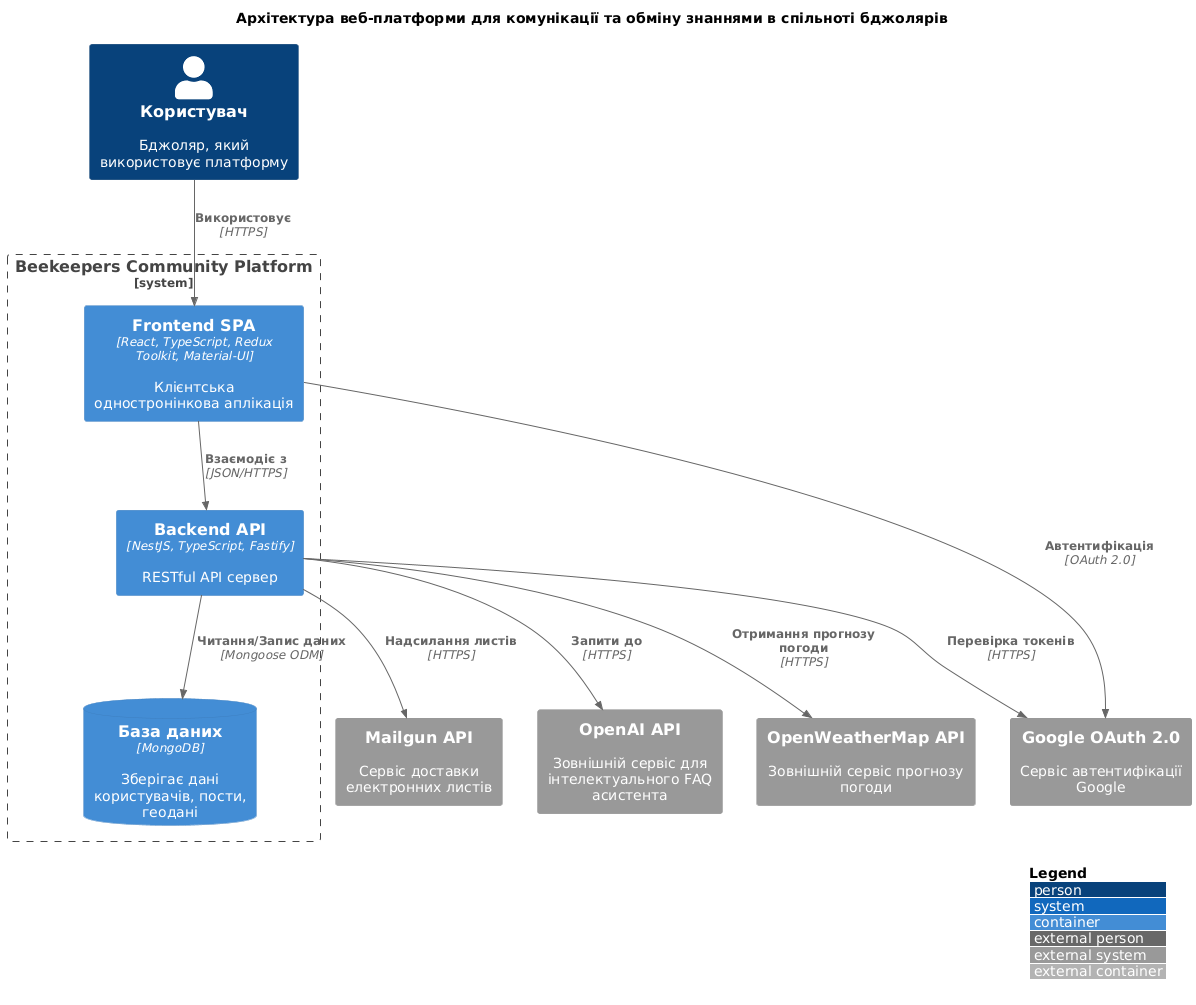
\includegraphics[width=0.7\textwidth]{images/system_architecture.png} % TODO: Add actual diagram
%   \fbox{Placeholder for High-Level System Architecture Diagram}
%   \caption{Загальна архітектура системи}
%   \label{fig:system_architecture}
% \end{figure}

\subsection{Архітектура фронтенду}
Клієнтська частина розроблена з використанням бібліотеки React та TypeScript. Управління станом реалізовано за допомогою Redux Toolkit, зокрема RTK Query для взаємодії з API та кешування даних. Навігація між сторінками забезпечується React Router. Для побудови користувацького інтерфейсу використано бібліотеку компонентів Material-UI (MUI), що дозволяє створювати адаптивні та візуально привабливі інтерфейси. Інтернаціоналізація реалізована за допомогою i18next та react-i18next. Картографічний функціонал побудований на базі Leaflet та React-Leaflet.
Структура проекту включає розділення на компоненти (загального призначення та специфічні для функціоналу), сторінки, сервіси (API-зрізи RTK Query), хуки, контексти та утиліти.

\subsection{Архітектура бекенду}
Серверна частина розроблена на платформі Node.js з використанням фреймворку NestJS та TypeScript. Архітектура є модульною, де кожен функціональний блок (наприклад, автентифікація, користувачі, форум, карта) виділений в окремий модуль. Кожен модуль містить контролери (обробка HTTP-запитів), сервіси (бізнес-логіка) та DTO (Data Transfer Objects) для валідації вхідних даних. Для взаємодії з базою даних MongoDB використовується ODM Mongoose. Автентифікація реалізована за допомогою Passport.js (JWT, локальна стратегія, Google OAuth). Для автоматичної генерації документації API використовується Swagger (OpenAPI). Застосунок працює на базі веб-сервера Fastify для підвищення продуктивності.

\subsection{Схема бази даних}
База даних MongoDB зберігає дані у вигляді колекцій документів. Основні колекції включають:
\begin{itemize}
    \item \texttt{users}: інформація про користувачів (email, хеш паролю, ім'я користувача, профільні дані, статус верифікації, токени, геодані тощо).
    \item \texttt{forumposts}: пости на форумі (заголовок, зміст, автор, коментарі, лайки).
    \item \texttt{hives}: дані про вулики (назва, нотатки, геокоординати GeoJSON Point, власник).
    \item \texttt{fields}: дані про поля (назва, тип культури, періоди цвітіння та обробки, геометрія GeoJSON Polygon, власник).
    \item (Інші колекції, якщо є, наприклад, для бази знань, подій).
\end{itemize}
Для геопросторових даних (координати вуликів та геометрія полів) використовуються відповідні індекси \texttt{2dsphere} для ефективних геозапитів.
% \begin{figure}[H]
%   \centering
%   % 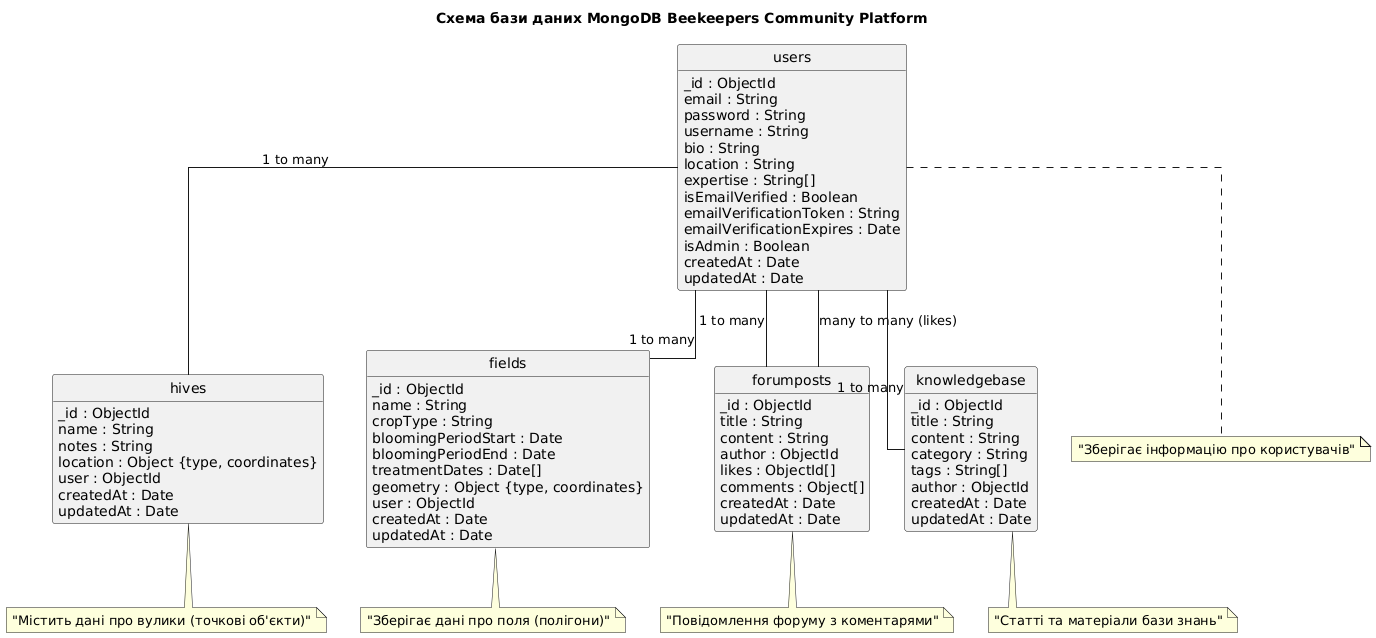
\includegraphics[width=\textwidth]{images/db_schema.png} % TODO: Add actual ERD/schema diagram
%   \fbox{Placeholder for Database Schema Diagram}
%   \caption{Логічна схема бази даних}
%   \label{fig:db_schema}
% \end{figure}

\section{Проектування UI/UX}
\label{sec:ui_ux}
Проектування користувацького інтерфейсу (UI) та досвіду взаємодії (UX) було спрямоване на створення інтуїтивно зрозумілої, зручної та візуально привабливої платформи. Основним інструментом для реалізації UI стала бібліотека компонентів Material-UI, яка надає широкий набір готових елементів дизайну, що відповідають сучасним стандартам Material Design. 

Ключові рішення:
\begin{itemize}
    \item \textbf{Адаптивний дизайн:} Забезпечення коректного відображення та функціонування на різних пристроях (десктопи, планшети, мобільні телефони).
    \item \textbf{Інтуїтивна навігація:} Використання бічної панелі навігації для доступу до основних розділів сайту та чіткої ієрархії сторінок.
    \item \textbf{Консистентність інтерфейсу:} Дотримання єдиного стилю оформлення елементів на всіх сторінках застосунку.
    \item \textbf{Інтерактивність:} Надання користувачам можливості легко взаємодіяти з елементами, такими як карта, форми, кнопки.
    \item \textbf{Зворотний зв'язок:} Інформування користувача про результати його дій (успіх, помилка, процес завантаження) за допомогою повідомлень та індикаторів.
\end{itemize}
% TODO: Include wireframes or mockups if available (can be in appendix). 

\subsubsection{Вимоги до форуму}
\begin{itemize}
    \item Реєстрація користувачів з верифікацією електронної пошти.
    \item Автентифікація (логін/пароль, можливість входу через Google OAuth).
    \item Зберігання даних користувачів (email, хеш паролю, ім'я користувача, роль, інформація про пасіку за бажанням).
    \item Управління профілем користувача.
    \item Відновлення паролю.
\end{itemize}

\subsubsection{Вимоги до бази знань}
\begin{itemize}
    \item Створення, редагування та видалення статей/ресурсів адміністраторами.
    \item Категоризація та тегування матеріалів.
    \item Пошук по базі знань.
    \item Система коментарів до статей (за бажанням).
    \item Рейтинг статей (за бажанням).
\end{itemize}

\subsubsection{Загальні нефункціональні вимоги}
\begin{itemize}
    \item \textbf{Безпека:} Захист від основних веб-вразливостей (XSS, CSRF, SQL/NoSQL ін'єкції), безпечне зберігання паролів, використання HTTPS.
    \item \textbf{Продуктивність:} Швидке завантаження сторінок та відгук інтерфейсу.
    \item \textbf{Масштабованість:} Архітектура повинна дозволяти додавання нового функціоналу та витримувати зростання кількості користувачів.
    \item \textbf{Надійність:} Система повинна бути доступною та стабільно працювати.
    \item \textbf{Зручність використання (Usability):} Інтуїтивно зрозумілий та легкий у використанні інтерфейс.
    \item \textbf{Адаптивність (Responsiveness):} Коректне відображення на різних пристроях (десктопи, планшети, мобільні телефони).
    \item \textbf{Інтернаціоналізація (i18n):} Підтримка української та англійської мов інтерфейсу.
    \item \textbf{Зворотний зв'язок:} Інформування користувача про результати його дій, помилки.
\end{itemize}    % System Design
% --- Chapter 3: Implementation ---
\chapter{Реалізація системи}
\label{ch:implementation}

\section{Огляд процесу розробки}
\label{sec:dev_process}
% TODO: Describe development methodology (e.g., Agile, Waterfall), tools used (Git, VS Code, Docker), and workflow.
Розробка веб-платформи для комунікації та обміну знаннями в спільноті бджолярів \textit{Beekeepers Community Platform} велася з використанням гнучких підходів, що дозволяли ітеративно додавати функціонал та вносити корективи. Основними інструментами розробки були Visual Studio Code як інтегроване середовище розробки, Git для системи контролю версій (з використанням GitHub для хостингу репозиторію), Docker та Docker Compose для контейнеризації та управління середовищем розробки та розгортання. Робочий процес включав регулярні коміти, розробку у функціональних гілках (за потреби) та тестування ключових функцій на локальному середовищі перед розгортанням.

\section{Організація коду}
\label{sec:code_organization}
Структура коду проекту організована для забезпечення модульності, легкості підтримки та масштабування.

\subsection{Структура проекту фронтенду}
Клієнтська частина (директорія \texttt{client/}) розроблена на React з використанням Vite як інструменту для збірки. Основні директорії в \texttt{src/}:
\begin{itemize}
    \item \texttt{components/}: Містить UI компоненти, розділені за функціональними ознаками (наприклад, \texttt{forum/}, \texttt{map/}, загальні компоненти).
    \item \texttt{pages/}: Компоненти, що відповідають за окремі сторінки застосунку (наприклад, \texttt{Home.tsx}, \texttt{Forums.tsx}, \texttt{MapPage.tsx}).
    \item \texttt{services/} (або \texttt{store/api/}): API-зрізи (slices) для RTK Query, що описують взаємодію з бекенд API (наприклад, \texttt{authApi.ts}, \texttt{forumApi.ts}, \texttt{mapApi.ts}).
    \item \texttt{store/}: Конфігурація Redux store (\texttt{store.ts}).
    \item \texttt{context/}: React Context API для управління глобальним станом, таким як автентифікація (\texttt{AuthContext.tsx}).
    \item \texttt{hooks/}: Спеціалізовані React хуки.
    \item \texttt{types/}: Загальні TypeScript типи та інтерфейси.
    \item \texttt{locales/}: Файли перекладів для інтернаціоналізації (\texttt{en/translation.json}, \texttt{uk/translation.json}).
    \item \texttt{utils/}: Допоміжні функції та утиліти.
    \item \texttt{App.tsx}: Головний компонент застосунку, що налаштовує маршрутизацію.
    \item \texttt{index.tsx} (або \texttt{main.tsx}): Вхідна точка застосунку.
\end{itemize}

\subsection{Структура проекту бекенду}
Серверна частина (директорія \texttt{server/}) розроблена на NestJS. Проект структурований за модульним принципом:
\begin{itemize}
    \item \texttt{src/}: Містить основний код застосунку.
    \item \texttt{src/MODULE\_NAME/}: Кожен функціональний блок (наприклад, \texttt{auth/}, \texttt{users/}, \texttt{forum/}, \texttt{hives/}, \texttt{fields/}, \texttt{health/}, \texttt{email/}) виділений в окремий модуль NestJS.
    \item Кожен модуль зазвичай містить:
        \begin{itemize}
            \item \texttt{*.module.ts}: Файл визначення модуля.
            \item \texttt{*.controller.ts}: Контролер, що обробляє запити за протоколом передачі гіпертексту (Hypertext Transfer Protocol, HTTP).
            \item \texttt{*.service.ts}: Сервіс, що інкапсулює бізнес-логіку.
            \item \texttt{schemas/}: Mongoose схеми для визначення структури даних MongoDB.
            \item \texttt{dto/}: Об'єкти передачі даних (Data Transfer Objects, DTOs) для валідації вхідних даних.
            \item \texttt{guards/}, \texttt{strategies/}, \texttt{decorators/}, \texttt{types/} (для специфічних типів модуля, наприклад, в \texttt{auth/}).
        \end{itemize}
    \item \texttt{src/main.ts}: Вхідна точка серверного застосунку, ініціалізація NestJS та Fastify.
    \item \texttt{src/app.module.ts}: Кореневий модуль застосунку.
\end{itemize}

\subsection{Проектування API}
Прикладний програмний інтерфейс (Application Programming Interface, API) спроектовано за принципами RESTful (Representational State Transfer). Всі кінцеві точки (ендпоінти) мають префікс \texttt{/api/v1/}, що забезпечує версіонування. Для валідації даних, що надходять від клієнта, використовуються об'єкти передачі даних (DTO) з декораторами \texttt{class-validator}. Документація API автоматично генерується за допомогою Swagger (OpenAPI) і доступна на ендпоінті \texttt{/docs} (у середовищі розробки), що спрощує тестування та інтеграцію.

\section{Опис ключових компонентів та модулів}
\label{sec:key_components}

\subsection{Автентифікація та авторизація}
Система автентифікації реалізована з використанням Passport.js. Підтримуються:
\begin{itemize}
    \item \textbf{Локальна стратегія:} Автентифікація за логіном (email) та паролем. Паролі зберігаються у хешованому вигляді (з використанням \texttt{crypto.pbkdf2Sync}).
    \item \textbf{JWT (JSON Web Tokens):} Використовуються для авторизації користувачів після успішного входу. Генеруються access та refresh токени.
    \item \textbf{Верифікація Email:} При реєстрації користувачу надсилається лист з унікальним токеном для підтвердження електронної пошти. Доступ до функціоналу обмежений до верифікації. Термін дії токена -- 1 година.
    \item \textbf{Повторне надсилання листа верифікації:} Реалізовано можливість для користувача запросити повторне надсилання листа для верифікації email, якщо попередній токен сплив або лист не було отримано. Цей функціонал включає новий ендпоінт API (\texttt{/auth/resend-verification-email}) та відповідний інтерфейс на сторінці верифікації (\texttt{VerifyEmailPage.tsx}).
    \item \textbf{Google OAuth 2.0:} Реалізовано можливість входу та реєстрації через обліковий запис Google. При натисканні кнопки "Увійти через Google" на сторінці входу (див. рисунок \ref{fig:login_page}), користувач перенаправляється на сторінку автентифікації Google. Після надання згоди, Google перенаправляє користувача назад до застосунку з авторизаційним кодом. Серверна частина обмінює цей код на токени доступу та інформацію про профіль користувача Google (email, ім\'я, фото). Бекенд-сервіс (\texttt{AuthService}, метод \texttt{findOrCreateGoogleUser}) перевіряє, чи існує користувач з таким email. Якщо так, користувач автентизується. Якщо ні, створюється новий обліковий запис, email автоматично позначається як верифікований, а для внутрішніх потреб генерується випадковий пароль (оскільки прямий вхід за паролем для таких акаунтів не передбачений). Після цього для користувача генеруються стандартні JWT (access та refresh токени) для подальшої роботи з платформою. Такий підхід спрощує процес реєстрації та входу для користувачів, підвищуючи зручність використання платформи.
    \item \textbf{Захист маршрутів (Guards):} \texttt{JwtAuthGuard} використовується для захисту ендпоінтів, що вимагають автентифікації. \texttt{LocalAuthGuard} використовується для обробки локального входу.
\end{itemize}

Для нових користувачів передбачено процес реєстрації, інтерфейс якого показаний на рисунку \ref{fig:registration_form}. Користувачу необхідно надати свою електронну адресу, обрати ім\'я користувача (username) та створити пароль. Після відправки форми, серверна частина виконує валідацію наданих даних. У випадку успішної валідації, створюється новий обліковий запис, пароль зберігається у хешованому вигляді, а для підтвердження електронної пошти генерується унікальний токен верифікації, який надсилається користувачу на вказану адресу. Цей крок є обов\\'язковим перед тим, як користувач зможе повноцінно увійти до системи та отримати доступ до її функціоналу.

\begin{figure}[htbp]
    \centering
    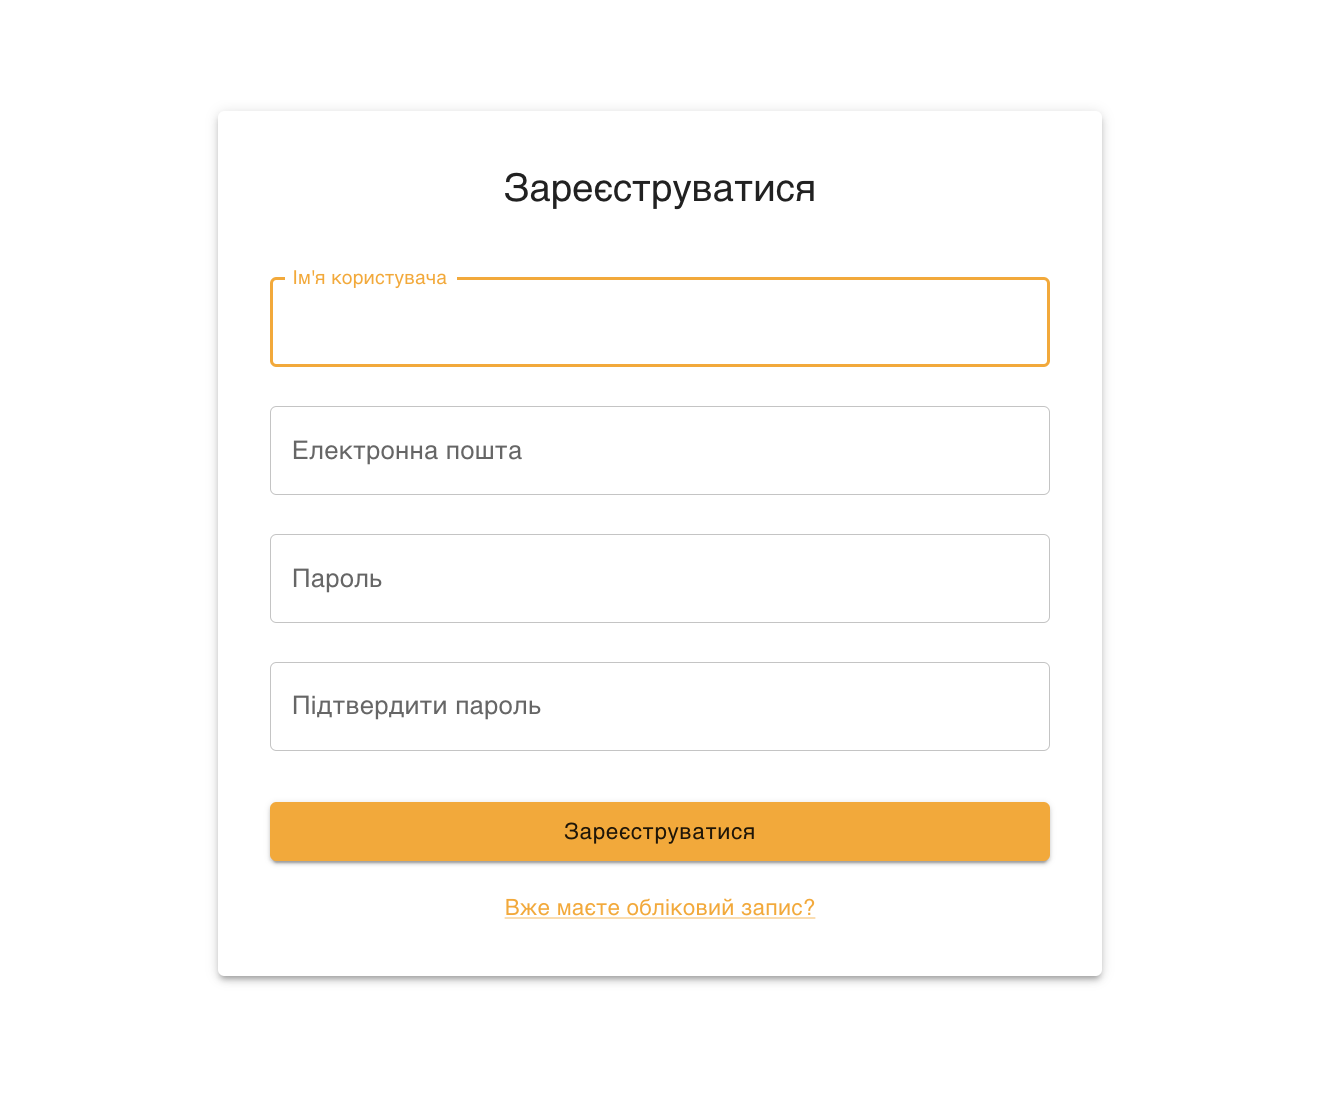
\includegraphics[width=0.6\textwidth]{practice_report/images/registration_form.png}
    \caption{Інтерфейс форми реєстрації нового користувача}
    \label{fig:registration_form}
\end{figure}

Детальна послідовність кроків, що включає як початкову реєстрацію, так і наступний етап верифікації електронної пошти через отриманий лист, ілюструється на діаграмі послідовності на рисунку \ref{fig:local_registration_flow}.

\begin{figure}[htbp]
    \centering
    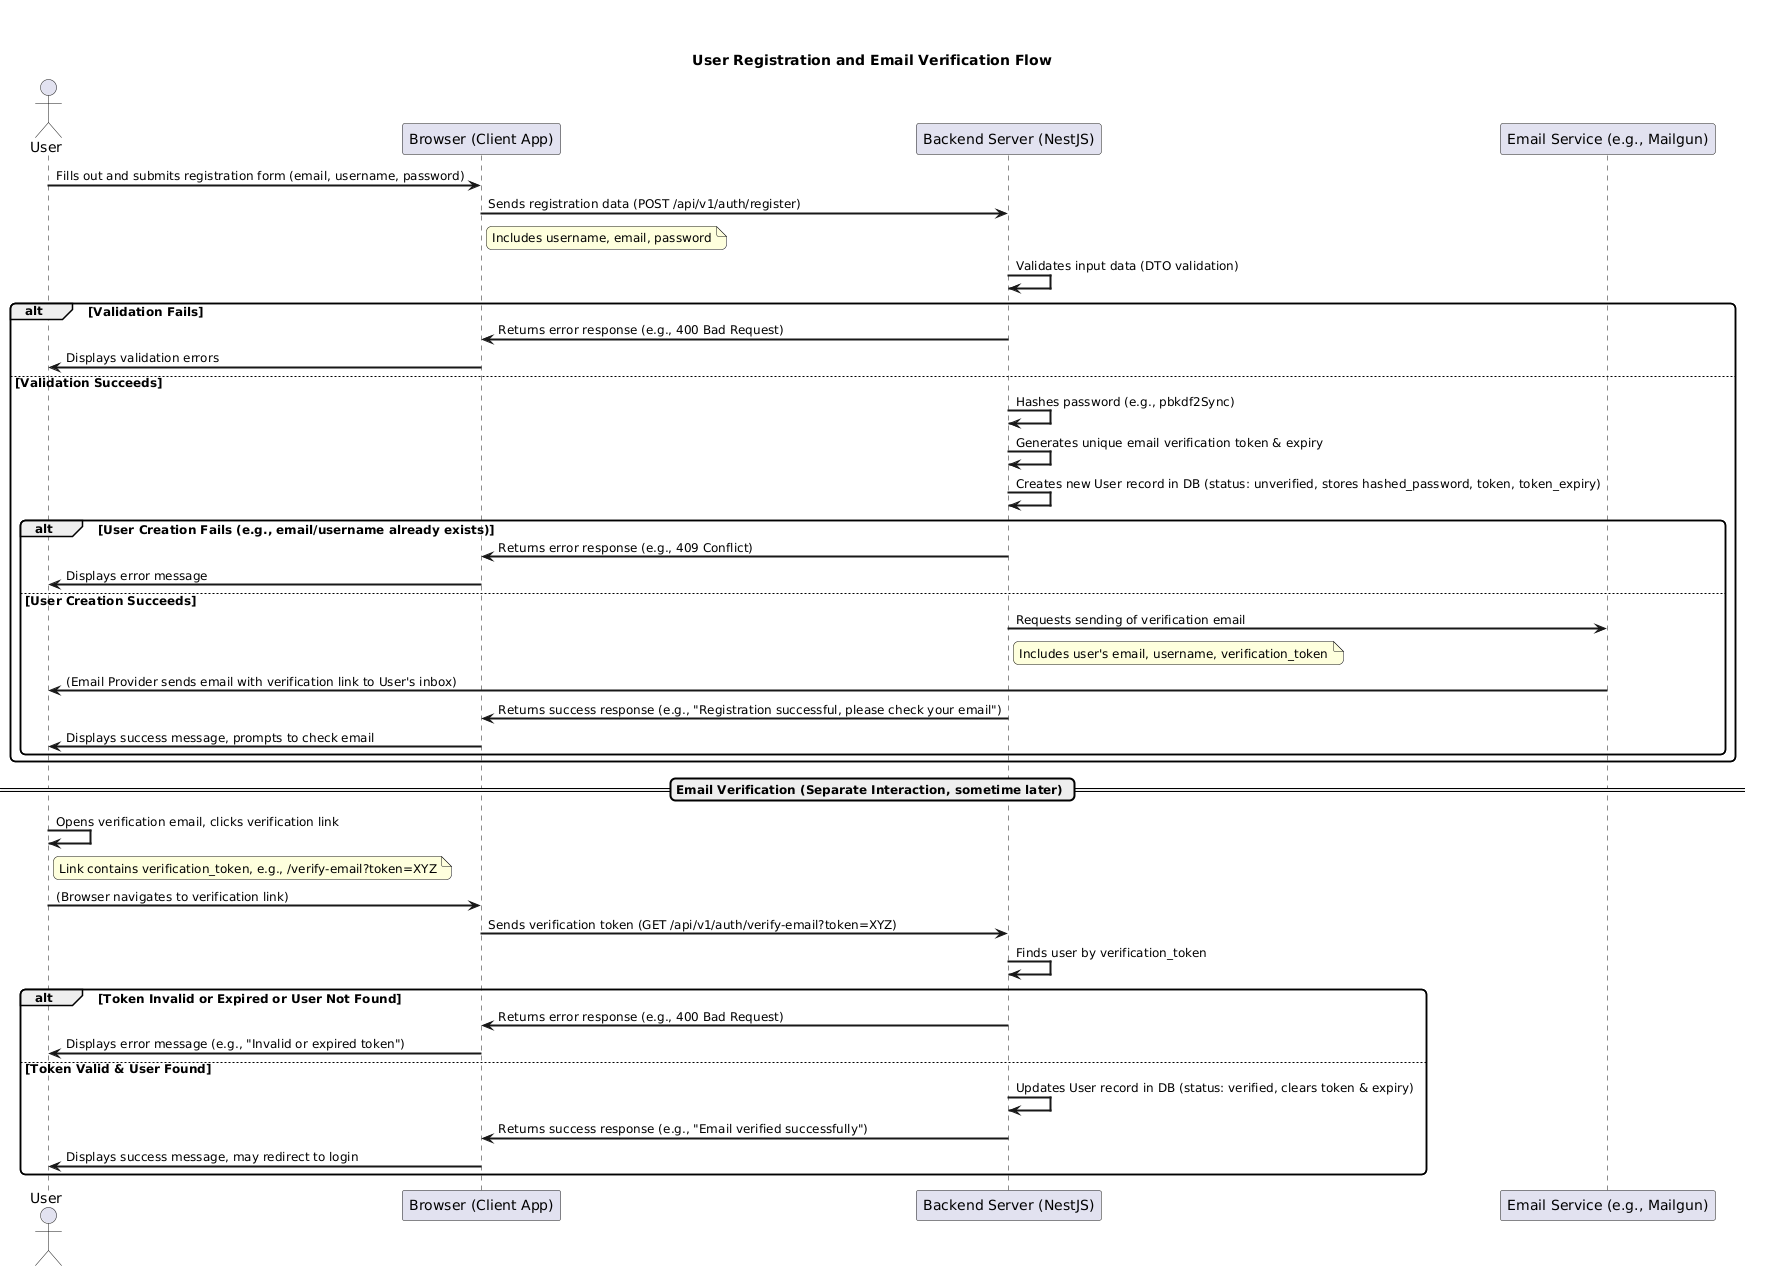
\includegraphics[width=\textwidth]{practice_report/images/local_registration_flow.png}
    \caption{Діаграма послідовності для реєстрації користувача та верифікації email}
    \label{fig:local_registration_flow}
\end{figure}

Центральним елементом процесу входу користувача є сторінка автентифікації, зображена на рисунку \ref{fig:login_page}. Інтерфейс надає поля для введення електронної пошти та пароля, кнопку для надсилання форми, а також посилання для переходу на сторінку реєстрації та кнопку для автентифікації через обліковий запис Google (використовуючи протокол OAuth 2.0). Після успішного введення облікових даних (або успішної автентифікації через Google) та їх перевірки на серверній стороні, користувач отримує доступ до захищених ресурсів платформи. Детальніше взаємодія між компонентами системи під час автентифікації, зокрема через Google, показана на діаграмі послідовності на рисунку \ref{fig:google_oauth_flow}.

\begin{figure}[htbp]
    \centering
    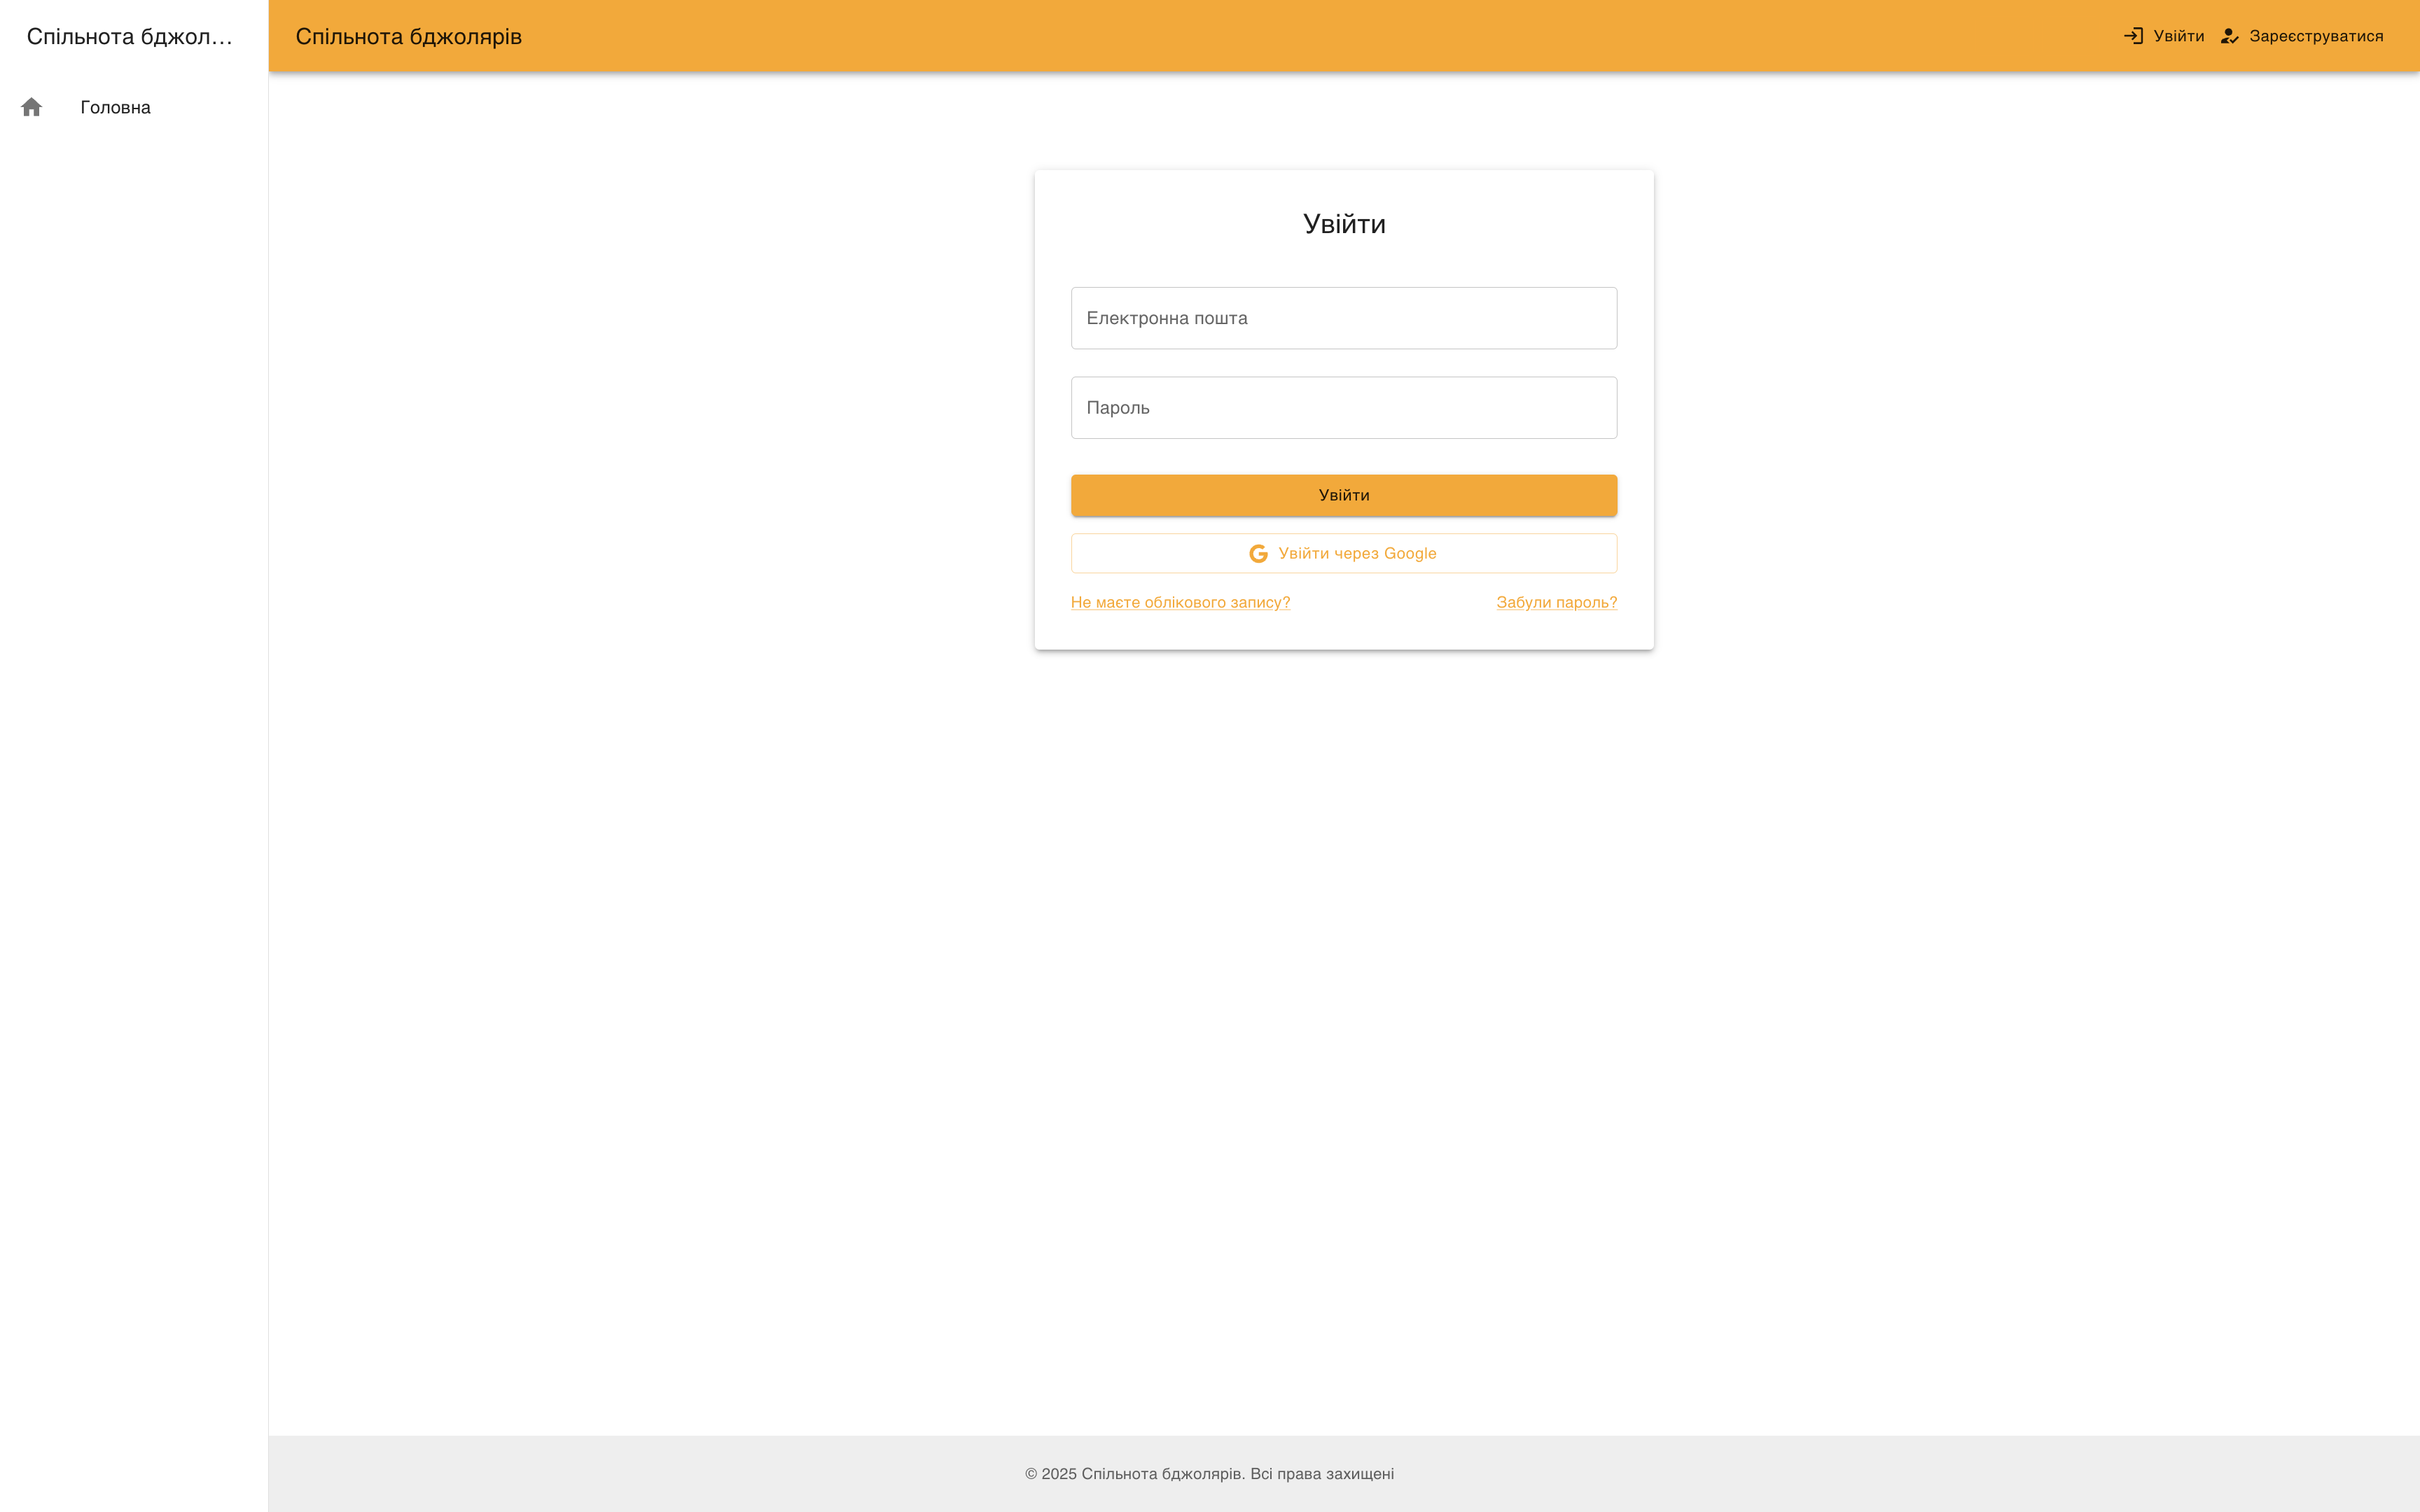
\includegraphics[width=0.8\textwidth]{practice_report/images/login_page.png}
    \caption{Інтерфейс сторінки входу до системи}
    \label{fig:login_page}
\end{figure}

Послідовність кроків, що виконуються під час автентифікації користувача за допомогою сервісу Google OAuth 2.0, включаючи взаємодію між клієнтом, серверною частиною платформи та сервером автентифікації Google, детально ілюстрована на рисунку \ref{fig:google_oauth_flow}.

\begin{figure}[htbp]
    \centering
    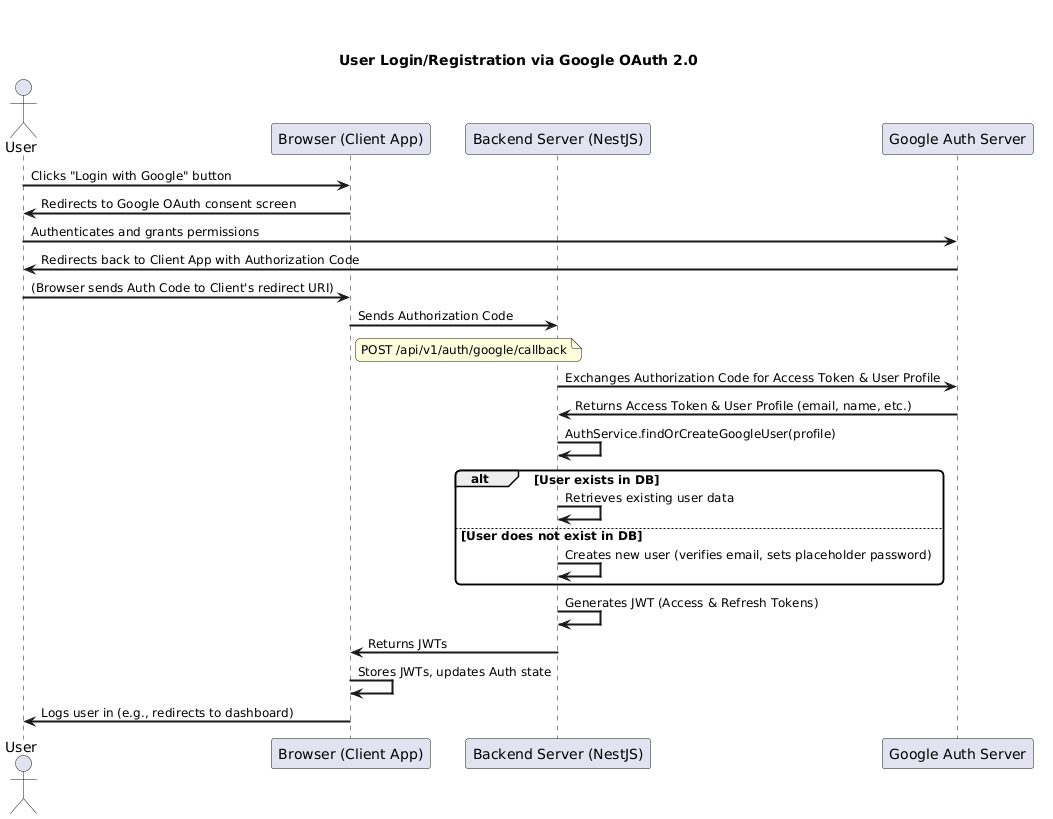
\includegraphics[width=\textwidth]{practice_report/images/google_oauth_flow.png}
    \caption{Послідовність дій при автентифікації через Google OAuth 2.0}
    \label{fig:google_oauth_flow}
\end{figure}

\subsection{Форум}
Модуль форуму дозволяє користувачам створювати теми для обговорення, залишати повідомлення та коментарі, а також висловлювати свою думку за допомогою лайків. Дані зберігаються в колекції \texttt{forumposts}. Фронтенд реалізований з використанням компонентів для списку постів, окремого поста та форми створення нового поста. Взаємодія з бекендом відбувається через відповідні API ендпоінти, реалізовані в \texttt{ForumController} та \texttt{ForumService}.

\subsection{База знань}
Модуль бази знань (на даний момент з демонстраційними даними на клієнті) передбачає зберігання та відображення статей, посібників та інших корисних матеріалів для бджолярів. Планується розширення функціоналу для управління контентом через адміністративну панель та реалізація повноцінного API для роботи з ресурсами бази знань.

\subsection{Інтеграція інтерактивної карти}
Одним з ключових функціональних блоків є інтерактивна карта, реалізована за допомогою Leaflet та React-Leaflet на фронтенді та GeoJSON з індексами \texttt{2dsphere} на бекенді (MongoDB). Компонент \texttt{MapPage.tsx} є центральним для цієї функціональності.

\subsubsection{Управління вуликами (Hives)}
Користувачі платформи мають можливість візуалізувати та управляти своїми вуликами безпосередньо на інтерактивній карті. Загальний вигляд розміщення вуликів на карті, включаючи їх маркери та спливаючі вікна з детальною інформацією, представлено на рисунку \ref{fig:map_hives_demo}.

\begin{figure}[htbp]
    \centering
    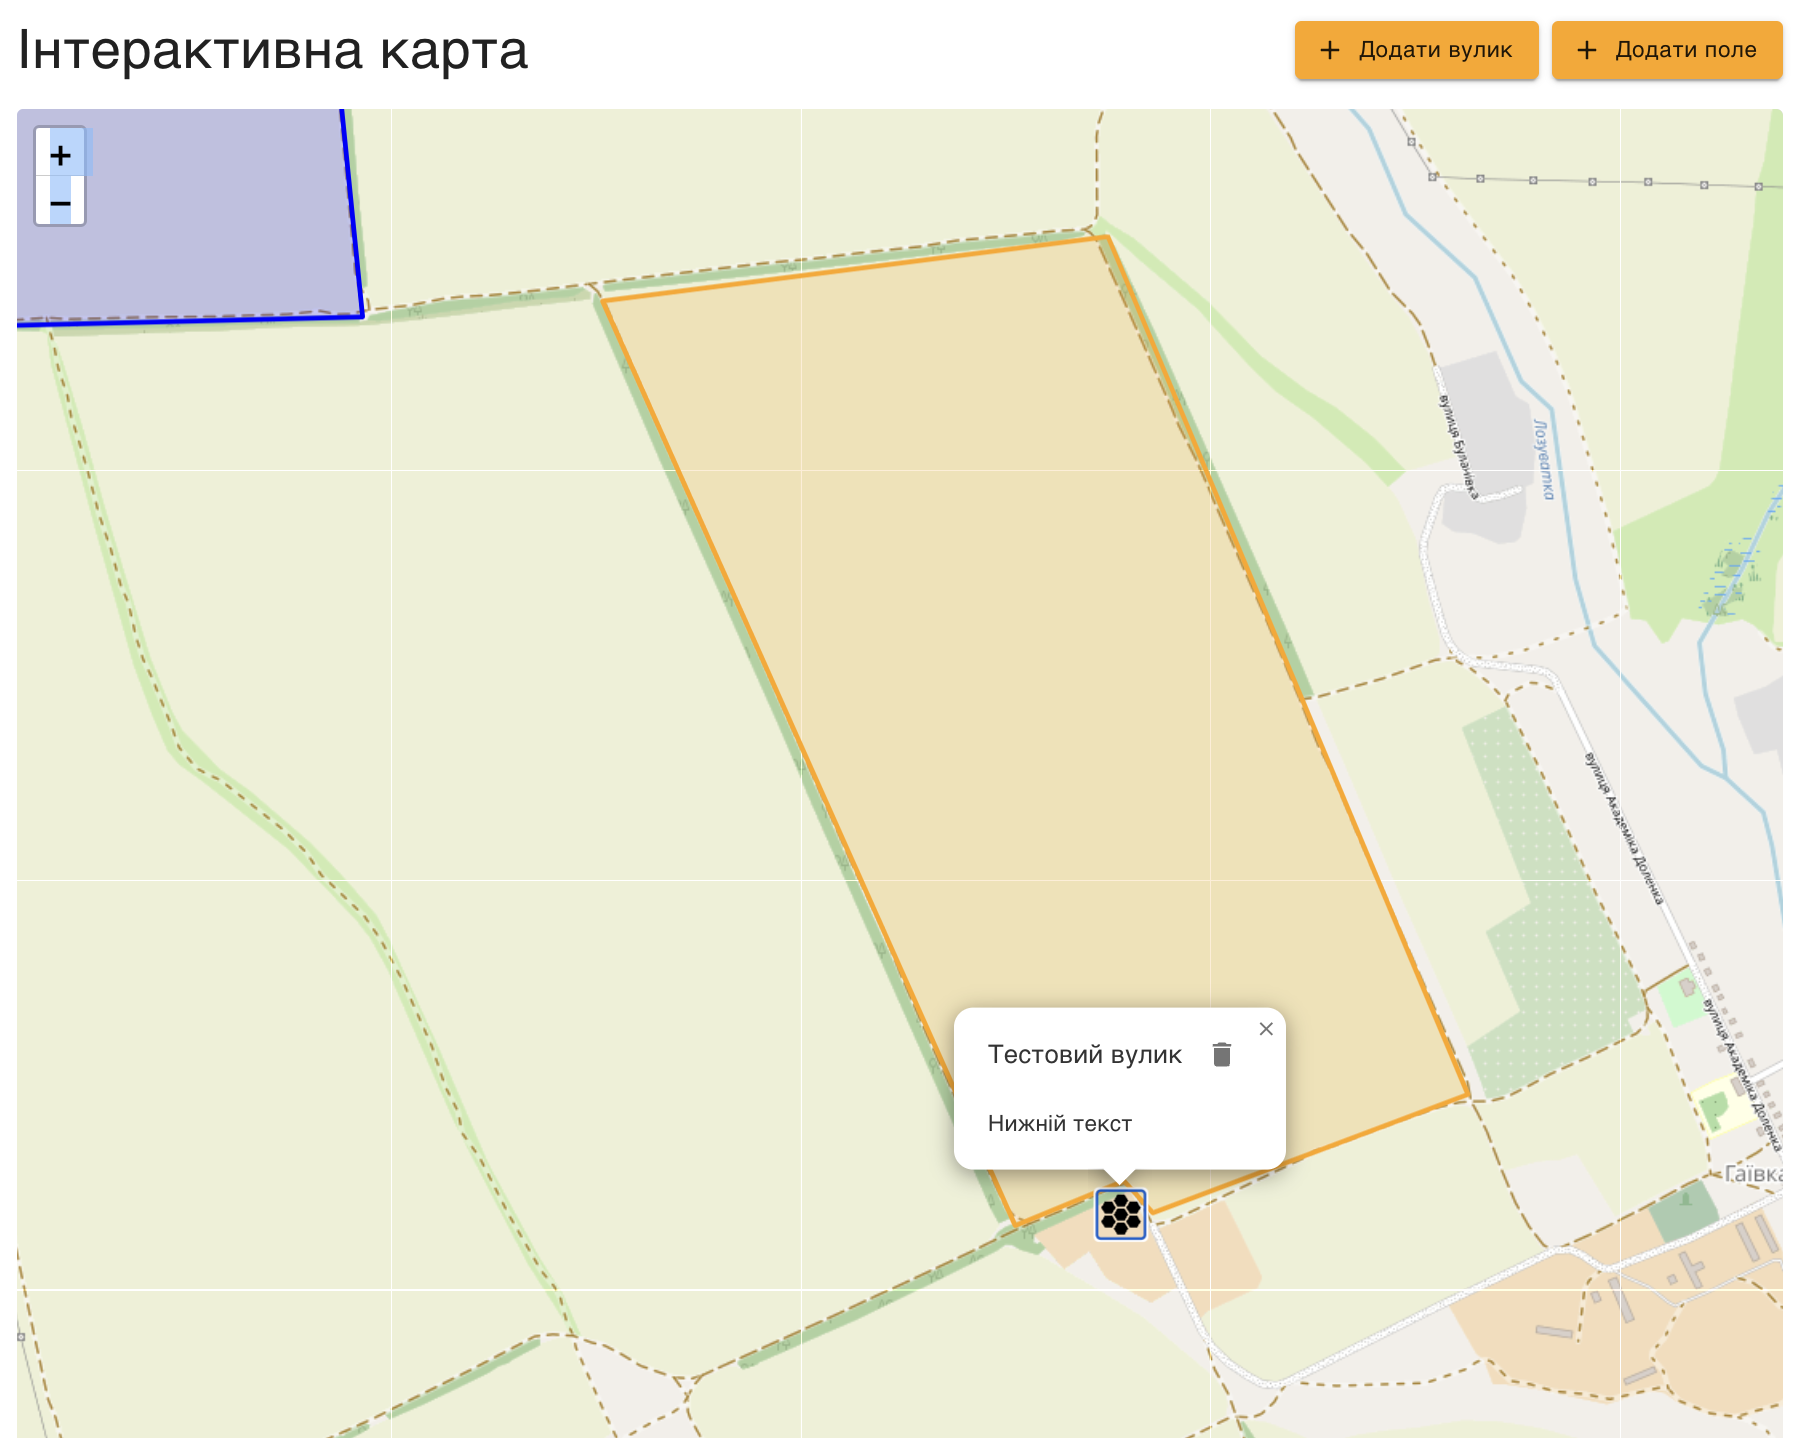
\includegraphics[width=0.8\textwidth]{practice_report/images/map_hives_demo.png}
    \caption{Демонстрація відображення вуликів на інтерактивній карті}
    \label{fig:map_hives_demo}
\end{figure}

\begin{itemize}
    \item \textbf{Додавання вуликів:} Користувачі можуть додавати на карту точкові маркери для позначення вуликів. Через діалогове вікно \texttt{AddHiveDialog.tsx} вказуються назва та нотатки. Геолокація визначається кліком на карті. Дані надсилаються на бекенд за допомогою RTK Query мутації \texttt{useAddHiveMutation}.
    
    \item \textbf{Відображення вуликів з кастомними іконками:} 
    Стандартні маркери бібліотеки Leaflet є досить загальними. Для покращення візуального сприйняття та тематичної відповідності було реалізовано відображення вуликів на карті за допомогою кастомних іконок. В якості візуального образу було обрано іконку \texttt{HiveIcon} з бібліотеки Material-UI, що забезпечує стилістичну єдність з іншими елементами інтерфейсу платформи. 
    
    Оскільки Leaflet очікує HTML-рядок або DOM-елемент для кастомних маркерів через \texttt{L.divIcon}, а \texttt{HiveIcon} є React-компонентом, було застосовано наступне рішення. За допомогою функції \texttt{ReactDOMServer.renderToString()} з пакету \texttt{react-dom/server} (яка зазвичай використовується для серверного рендерингу) React-компонент іконки перетворюється на статичний HTML-рядок на стороні клієнта. Цей рядок потім передається у властивість \texttt{html} об'єкта конфігурації \texttt{L.divIcon}. 
    
    При створенні кастомної іконки також налаштовуються важливі параметри \texttt{L.divIcon}, такі як \texttt{className} (для можливості додаткової стилізації за допомогою каскадних таблиць стилів (Cascading Style Sheets, CSS)), \texttt{iconSize} (розмір іконки), \texttt{iconAnchor} (точка прив'язки іконки до географічних координат, щоб вістря іконки вказувало на точне місце), та \texttt{popupAnchor} (позиціонування спливаючого вікна відносно іконки). Сформований таким чином об'єкт \texttt{hiveLeafletIcon} потім передається у пропс \texttt{icon} компонента \texttt{<Marker>} з бібліотеки React-Leaflet. Такий підхід дозволив ефективно інтегрувати React-компоненти Material-UI в картографічний контекст Leaflet, забезпечуючи кращий користувацький досвід та візуальну привабливість карти.

    \item \textbf{Видалення вуликів:} Користувачі можуть видаляти свої вулики. У спливаючому вікні (Popup) маркера вулика розміщена кнопка видалення. Натискання на неї активує діалогове вікно для підтвердження дії. Після підтвердження, мутація \texttt{useDeleteHiveMutation} з RTK Query відправляє запит на бекенд для видалення відповідного запису з колекції \texttt{hives}.
    \item \textbf{Перегляд інформації:} У спливаючому вікні (Popup) кожного вулика відображається його назва та нотатки.
\end{itemize}

\subsubsection{Управління полями (Fields)}
Аналогічно до вуликів, користувачі можуть додавати, переглядати та управляти інформацією про сільськогосподарські поля. На рисунку \ref{fig:map_fields_demo} показано, як поля відображаються у вигляді полігонів, разом зі спливаючими вікнами, що містять ключову інформацію, таку як тип культури та дати обробок.

\begin{figure}[htbp]
    \centering
    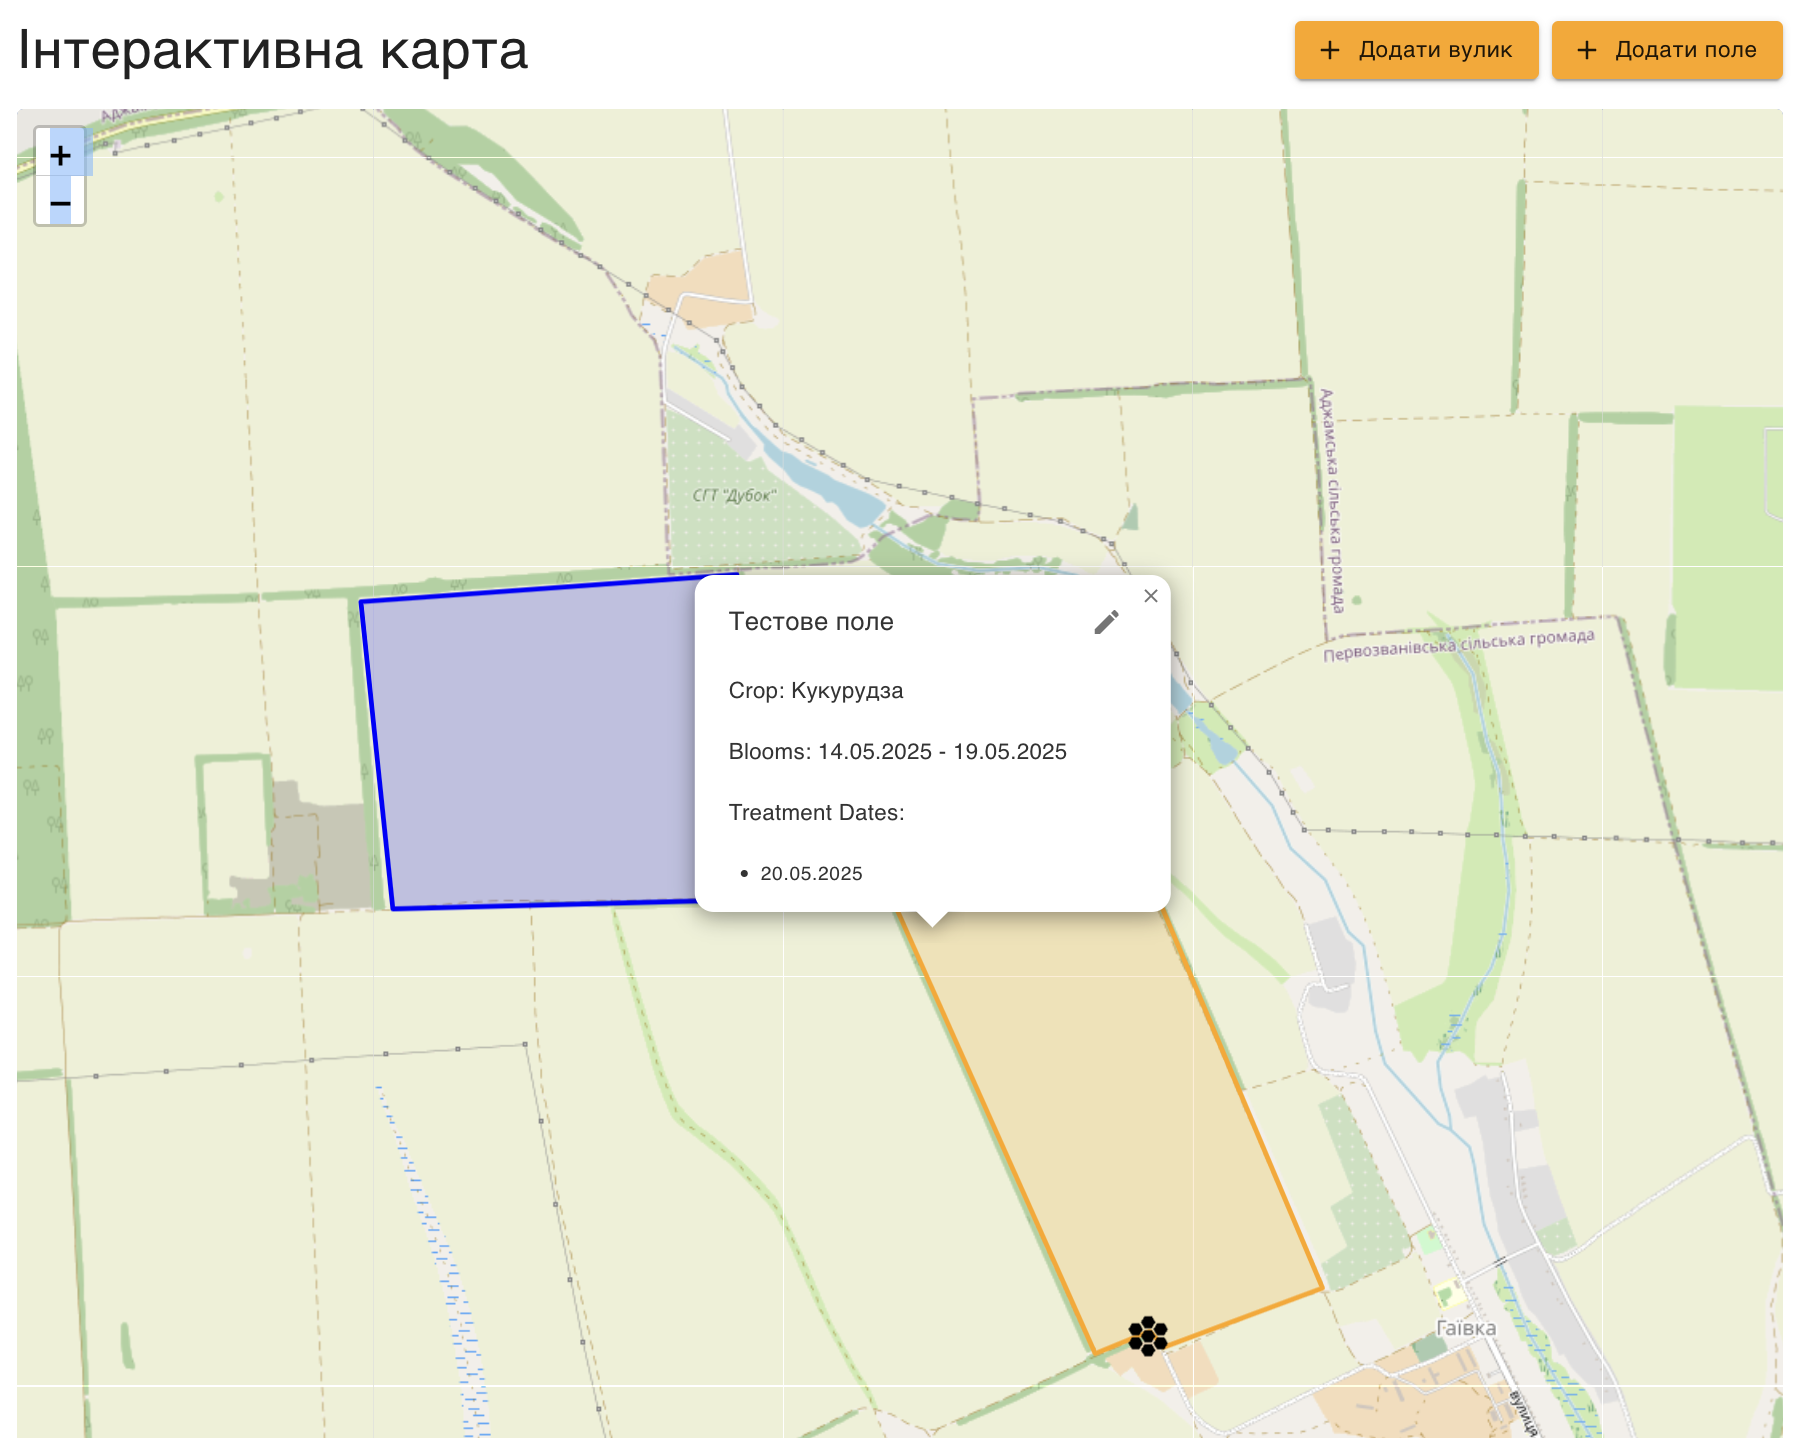
\includegraphics[width=0.8\textwidth]{practice_report/images/map_fields_demo.png}
    \caption{Демонстрація відображення полів на інтерактивній карті}
    \label{fig:map_fields_demo}
\end{figure}

\begin{itemize}
    \item \textbf{Додавання полів:} Користувачі можуть малювати полігони на карті для позначення полів. Діалогове вікно \texttt{AddFieldDialog.tsx} дозволяє вказати назву поля, тип культури, період цвітіння та список запланованих дат обробки. Геометрія полігону передається на бекенд у форматі GeoJSON. Використовується мутація \texttt{useAddFieldMutation}.
    
    \item \textbf{Відображення полів та візуалізація статусу обробки:} 
    Поля відображаються як полігони на карті за допомогою компонента \texttt{<Polygon>} з бібліотеки React-Leaflet. Ключовою особливістю є динамічна зміна кольору полігону для візуального інформування бджолярів про заплановані хімічні обробки полів, що можуть становити загрозу для бджіл. Ця логіка реалізована в компоненті \texttt{MapPage.tsx} у функції \texttt{getFieldTreatmentStatus}. 
    
    Функція приймає масив дат обробок для конкретного поля. Вона порівнює кожну дату обробки з поточною датою. Якщо обробка запланована на сьогодні, полю присвоюється червоний колір (високий ризик). Якщо обробка запланована протягом наступних семи днів (визначено константою \texttt{TREATMENT\_SOON\_DAYS}), полю присвоюється помаранчевий колір (середній ризик). В інших випадках використовується стандартний синій колір. Перевірка на "сьогодні" здійснюється за допомогою допоміжної функції \texttt{isSameDay}, яка порівнює рік, місяць та день двох дат. Результатом роботи \texttt{getFieldTreatmentStatus} є об'єкт, що містить властивість \texttt{color}, значення якої динамічно передається в атрибут \texttt{pathOptions} компонента \texttt{<Polygon>}. Для оптимізації та уникнення зайвих перерахунків при кожному рендері компонента, функція \texttt{getFieldTreatmentStatus} обгорнута в React хук \texttt{useMemo} (хоча в поточній реалізації без залежностей вона створюється один раз). Це забезпечує користувачам наочне та оперативне сповіщення про потенційні загрози.

    \item \textbf{Редагування метаданих полів:} 
    Для модифікації атрибутів існуючих полів було розроблено спеціалізований діалоговий компонент \texttt{EditFieldDialog.tsx}. Активація цього діалогу відбувається при натисканні користувачем кнопки редагування у спливаючому вікні (Popup) відповідного полігону поля на карті. Компонент отримує через пропси поточні дані поля (\texttt{initialData}), прапорець видимості (\texttt{open}), обробники закриття (\texttt{onClose}) та відправки форми (\texttt{onSubmit}), а також стан завантаження (\texttt{isLoading}) для індикації процесу взаємодії з API.
    
    Внутрішній стан форми (\texttt{formData}), що включає назву, тип культури, дати початку та кінця цвітіння, а також список дат обробки, управляється за допомогою хука \texttt{useState}. При відкритті діалогу або зміні \texttt{initialData}, хук \texttt{useEffect} відповідає за ініціалізацію стану форми даними обраного поля. Важливим аспектом є перетворення форматів дат: рядкові ISO-дати, отримані з бекенду, форматуються у вигляд \texttt{YYYY-MM-DD}, сумісний з HTML-елементами вводу типу \texttt{date}.
    
    Обробка змін у текстових полях форми реалізована через універсальний обробник \texttt{handleChange}. Для управління динамічним списком дат обробки передбачені окремі функції: \texttt{addTreatmentDate} для додавання нового поля вводу дати, \texttt{removeTreatmentDate} для видалення існуючого, та \texttt{handleTreatmentDateChange} для оновлення конкретної дати у списку. 
    
    При відправці форми функція \texttt{handleSubmit} виконує базову валідацію введених даних. Якщо валідація успішна, викликається переданий через пропси обробник \texttt{onSubmit} (визначений у \texttt{MapPage.tsx}). Цей обробник, у свою чергу, активує RTK Query мутацію \texttt{useUpdateFieldMutation}, передаючи ідентифікатор поля (\texttt{\_id}) та об'єкт \texttt{formData} з оновленими даними на сервер. Протягом виконання асинхронного запиту до API, пропс \texttt{isLoading} використовується для блокування елементів форми та відображення індикатора завантаження на кнопці збереження, забезпечуючи користувачеві зворотний зв'язок.

    \item \textbf{Перегляд інформації:} У спливаючому вікні (Popup) кожного поля відображається його назва, тип культури, період цвітіння та список дат обробки.
\end{itemize}

Бекенд надає відповідні CRUD (Create, Read, Update, Delete – Створити, Прочитати, Оновити, Видалити) API ендпоінти для управління вуликами та полями, забезпечуючи збереження, отримання, оновлення та видалення геопросторових об'єктів та їх метаданих (колекції \texttt{hives} та \texttt{fields} у MongoDB).

\subsection{Реалізація функціоналу адміністрування користувачів}
\label{subsec:admin_user_management}
Для забезпечення можливостей управління користувачами платформи було розроблено адміністративний функціонал, доступний лише користувачам з роллю адміністратора. Цей функціонал включає перегляд списку всіх користувачів та можливість зміни їх адміністративного статусу.

\subsubsection{Захист адміністративних маршрутів}
На серверній стороні доступ до адміністративних ендпоінтів контролюється за допомогою спеціалізованого NestJS Guard – \texttt{AdminGuard} (файл \texttt{server/src/auth/guards/admin.guard.ts}). Цей guard активується після успішної автентифікації користувача через \texttt{JwtAuthGuard}. \texttt{AdminGuard} перевіряє наявність поля \texttt{isAdmin} зі значенням \texttt{true} в об'єкті користувача, що додається до запиту \texttt{JwtAuthGuard}. Якщо користувач не є адміністратором, guard генерує виняток \texttt{ForbiddenException}, блокуючи доступ.

\subsubsection{Сервісні методи та контролери для управління користувачами}
У сервісі \texttt{UsersService} (\texttt{server/src/users/users.service.ts}) було додано два ключових методи для адміністративних потреб:
\begin{itemize}
    \item \texttt{findAllAdmin()}: Повертає повний список всіх документів користувачів з бази даних. На відміну від потенційних публічних методів отримання користувачів, цей метод призначений для надання адміністратору повного огляду.
    \item \texttt{updateUserAdminStatus(userIdToUpdate: string, isAdmin: boolean)}: Оновлює поле \texttt{isAdmin} для вказаного користувача. Метод знаходить користувача за \texttt{userIdToUpdate} та встановлює нове значення для його адміністративного статусу, повертаючи оновлений документ користувача.
\end{itemize}
Відповідні ендпоінти були додані до \texttt{UsersController} (\texttt{server/src/users/users.controller.ts}):
\begin{itemize}
    \item \texttt{GET /users/admin/all}: Викликає \texttt{usersService.findAllAdmin()} та захищений \texttt{JwtAuthGuard} і \texttt{AdminGuard}.
    \item \texttt{PATCH /users/admin/:userId/set-admin-status}: Приймає \texttt{userId} як параметр маршруту та тіло запиту типу \texttt{SetUserAdminStatusDto} (що містить поле \texttt{isAdmin: boolean}). Викликає \texttt{usersService.updateUserAdminStatus()} та також захищений обома guards.
\end{itemize}
Для валідації тіла запиту при зміні статусу адміністратора використовується DTO \texttt{SetUserAdminStatusDto} з відповідними декораторами \texttt{class-validator}.

\subsubsection{Клієнтська реалізація панелі адміністратора}
На клієнтській стороні було створено сторінку \texttt{AdminPage.tsx} (розташовану в \texttt{client/src/pages/}), яка слугує інтерфейсом для управління користувачами. Доступ до цієї сторінки контролюється на рівні компонента: перевіряється, чи поточний автентифікований користувач (отриманий за допомогою хука \texttt{useAuth} з \texttt{AuthContext}) має прапорець \texttt{isAdmin}, встановлений в \texttt{true}. Якщо користувач не є адміністратором, або дані про користувача ще завантажуються, відображається відповідне повідомлення про відмову в доступі або індикатор завантаження.

Для отримання списку всіх користувачів сторінка використовує RTK Query хук \texttt{useGetAllUsersAdminQuery} з \texttt{usersApi.ts}. Запит пропускається (опція \texttt{skip}), якщо поточний користувач не визначений як адміністратор. Отриманий список користувачів відображається за допомогою компонентів Material-UI \texttt{<List>}, \texttt{<ListItem>} та \texttt{<ListItemText>}, показуючи ім'я користувача, його email та ID. Поточний залогінений адміністратор візуально виділяється у списку.

Зміна адміністративного статусу користувача реалізована за допомогою компонента \texttt{<Switch>} (Material-UI) для кожного користувача у списку. Обробник \texttt{handleAdminStatusChange} викликається при зміні стану перемикача. Цей обробник ініціює RTK Query мутацію \texttt{useUpdateUserAdminStatusMutation}, передаючи ID користувача та нове значення статусу \texttt{isAdmin}. Для запобігання випадковій зміні власних прав, перемикач для поточного адміністратора деактивується. Після успішного виконання мутації (оновлення даних на сервері), викликається функція \texttt{refetch} (надана хуком \texttt{useGetAllUsersAdminQuery}) для оновлення списку користувачів на сторінці, що забезпечує актуальність відображених даних. Стани завантаження під час отримання списку (\texttt{isLoadingUsers}) та оновлення статусу (\texttt{isUpdatingStatus}) використовуються для відображення індикатора \texttt{<CircularProgress>}, надаючи користувачеві зворотний зв'язок про хід операцій. Текстові елементи на сторінці інтернаціоналізовані за допомогою хука \texttt{useTranslation} з \texttt{react-i18next}.

\subsection{Налаштування доставки транзакційних електронних листів}
\label{subsec:email_delivery}

Для забезпечення надійної та безпечної доставки транзакційних електронних листів (наприклад, для верифікації email), веб-платформа для комунікації та обміну знаннями в спільноті бджолярів \textit{Beekeepers Community Platform} інтегрується з сервісом Mailgun. Правильне налаштування системи доменних імен (Domain Name System, DNS) є критично важливим для доставки та відповідності сучасним галузевим стандартам, особливо тим, що висуваються великими провайдерами, такими як Google та Yahoo.

\subsubsection{Автентифікація домену}

Для автентифікації вихідних електронних листів до DNS-конфігурації домену проекту були додані наступні записи:

\begin{itemize}
    \item \textbf{SPF (Sender Policy Framework):} TXT-запис, що вказує, які поштові сервери мають право надсилати електронні листи від імені домену. Це допомагає запобігти несанкціонованим відправникам (спуфінгу).
    \item \textbf{DKIM (DomainKeys Identified Mail):} TXT-запис, що містить публічний криптографічний ключ. Вихідні листи підписуються приватним ключем Mailgun, а одержувачі можуть перевірити підпис за допомогою публічного ключа в DNS, забезпечуючи цілісність та автентичність повідомлення.
    \item \textbf{DMARC (Domain-based Message Authentication, Reporting, and Conformance):} TXT-запис, який інструктує приймаючі поштові сервери, як обробляти листи, що не пройшли перевірки SPF або DKIM.
        \begin{itemize}
            \item \textbf{Опції політики:}
                \begin{itemize}
                    \item \texttt{p=none}: Тільки моніторинг, без примусових дій.
                    \item \texttt{p=quarantine}: Відправляти листи, що не пройшли перевірку, до папки "Спам".
                    \item \texttt{p=reject}: Повністю блокувати листи, що не пройшли перевірку.
                \end{itemize}
            \item \textbf{Сучасна практика:} Через нові вимоги Google та Yahoo (з 2024 року), політика DMARC повинна бути встановлена щонайменше на \texttt{quarantine} або \texttt{reject} для використання у виробничому середовищі. Це захищає користувачів від фішингу та покращує доставку.
        \end{itemize}
\end{itemize}

\subsubsection{Поширення та верифікація DNS}

Після додавання необхідних записів, поширення змін у DNS може зайняти до 48 годин. Верифікація виконується за допомогою панелі керування Mailgun та сторонніх інструментів (наприклад, MXToolbox), щоб переконатися, що всі записи коректно опубліковані та доступні глобально.

\subsubsection{Безпека та відповідність стандартам}

\begin{itemize}
    \item \textbf{Відсутність жорстко закодованих облікових даних:} Усі API-ключі Mailgun та конфіденційні налаштування зберігаються у змінних середовища, а не в коді.
    \item \textbf{Постійний моніторинг:} Звіти DMARC надсилаються на визначену електронну адресу для моніторингу проблем автентифікації та потенційного зловживання.
    \item \textbf{Ескалація політики:} Проект спочатку використовує \texttt{p=none} для DMARC для моніторингу легітимного трафіку, а потім переходить до \texttt{quarantine} або \texttt{reject} для повної відповідності стандартам та захисту.
\end{itemize}

\subsubsection{Підсумкова таблиця DNS-записів}

\begin{table}[h!]
\centering
\begin{tabular}{|l|l|l|}
\hline
\textbf{Запис} & \textbf{Призначення} & \textbf{Приклад значення / Політика} \\
\hline
SPF    & Автентифікація відправника & \texttt{v=spf1 include:mailgun.org \~{}all} \\
DKIM   & Підпис повідомлення & (Публічний ключ, наданий Mailgun) \\
DMARC  & Політика та звіти & \texttt{v=DMARC1; p=quarantine; rua=mailto:admin@domain.com} \\
\hline
\end{tabular}
\caption{Приклади DNS-записів для автентифікації email.}
\label{tab:dns_records_email}
\end{table}

Така конфігурація гарантує, що всі вихідні електронні листи автентифіковані, знижуючи ризик спаму та фішингу та відповідаючи останнім вимогам основних поштових провайдерів. Вона також підтримує моніторинг та постійне вдосконалення безпеки електронної пошти.

\subsection{Реалізація інтелектуального FAQ-асистента}
\label{subsec:ai_faq_implementation}
Для надання користувачам швидких відповідей на поширені питання було реалізовано прототип інтелектуального FAQ-асистента, що використовує можливості великих мовних моделей (LLM), зокрема GPT-3.5-turbo від OpenAI \cite{openai_api}. Метою було дослідження потенціалу застосування LLM для покращення користувацького досвіду та оперативності надання інформації в рамках платформи.

\subsubsection{Серверна частина (Backend): Промпт-інжиніринг та взаємодія з OpenAI}
На бекенді, в модулі \texttt{FaqModule}, ключову роль відіграє \texttt{FaqService}. Цей сервіс відповідає за підготовку даних, конструювання промпту та взаємодію з API OpenAI.
\begin{itemize}
    \item \textbf{DTO запиту та Контролер:} Як і в інших модулях, використовується DTO \texttt{AskFaqDto} для валідації вхідного питання від користувача, яке надходить на ендпоінт \texttt{POST /api/v1/faq/ask}, оброблюваний \texttt{FaqController}.
    
    \item \textbf{Управління API-ключем:} API-ключ для доступу до OpenAI завантажується з конфігураційних файлів (змінних середовища) через \texttt{ConfigService}. Реалізовано перевірку наявності ключа при ініціалізації сервісу; у разі його відсутності, функціонал FAQ стає недоступним, про що логується попередження та інформується користувач при спробі запиту.

    \item \textbf{Побудова промпту – ядро логіки сервісу:}
    Якість відповіді LLM значною мірою залежить від якості та структури наданого промпту. У поточній реалізації прототипу застосовано наступний підхід до промпт-інжинірингу в методі \texttt{answerQuestion}:
    \begin{enumerate}
        \item \textbf{Формування контексту з ЧаПи (FAQ):} На даному етапі використовується статичний масив \texttt{FAQ\_DATA}, що містить пари «питання-відповідь». Перед відправкою до LLM, цей масив перетворюється на текстовий блок, де кожне питання та відповідь чітко позначені (наприклад, Q1:/A1:, Q2:/A2:). Це допомагає моделі розрізняти окремі елементи ЧаПи. 
        \textit{Обмеження поточного підходу до контексту:} Основне обмеження полягає в тому, що весь обсяг \texttt{FAQ\_DATA} включається в кожен запит. Зі зростанням кількості ЧаПи, це призведе до перевищення ліміту токенів, який підтримує обрана модель (наприклад, gpt-3.5-turbo має ліміт близько 4096 токенів для промпту та відповіді разом). Це робить поточне рішення не масштабованим для великих баз знань і слугує обґрунтуванням для впровадження семантичного пошуку в майбутньому.
        
        \item \textbf{Розробка системного повідомлення (System Prompt):} Системне повідомлення є критично важливим для керування поведінкою LLM. Для даного асистента воно було сформульовано таким чином, щоб чітко визначити роль моделі, обмежити джерело її знань та задати стиль відповіді:
        \begin{quote}
        \textit{Ви є корисним асистентом для платформи "Beekeepers Community Platform". Ваше завдання - відповідати на питання користувачів, базуючись ВИКЛЮЧНО на наданому контексті з ЧаПи (Часто Задаваних Питань). Якщо відповіді немає в контексті, чітко вкажіть, що ви не можете надати відповідь на основі наявної інформації. Не вигадуйте відповіді. Будьте коротким та чітким. Відповідайте українською мовою.}
        \end{quote}
        Ключові елементи цього промпту – вимога базуватися \textbf{виключно} на наданому контексті та інструкція щодо поведінки у випадку відсутності інформації – спрямовані на мінімізацію «галюцинацій» моделі (генерування неправдивої або нерелевантної інформації) та забезпечення того, що користувачі отримують відповіді, що стосуються саме платформи.
        
        \item \textbf{Конструювання фінального запиту до моделі:} Питання користувача, попередньо підготовлений контекст ЧаПи та системне повідомлення об'єднуються в структурований запит (у форматі повідомлень для Chat Completions API OpenAI), який надсилається до моделі. Це забезпечує чітке розділення інструкцій, контекстуальних даних та запиту користувача.
    \end{enumerate}

    \item \textbf{Взаємодія з OpenAI API та параметризація:}
    Для взаємодії з API використовується офіційна бібліотека \texttt{openai} для Node.js. Було обрано модель \texttt{gpt-3.5-turbo} як збалансований варіант за співвідношенням можливостей та вартості. Ключові параметри запиту до API включають:
    \begin{itemize}
        \item \texttt{model}: Назва використовуваної моделі.
        \item \texttt{messages}: Масив об'єктів, що включає системне повідомлення та повідомлення користувача (з контекстом та питанням).
        \item \texttt{temperature}: Встановлено на низьке значення (наприклад, 0.2 з діапазону 0 до 2) для зменшення випадковості та отримання більш детермінованих, фактологічних відповідей, що є бажаним для FAQ-системи.
        \item \texttt{max\_tokens}: Обмежує максимальну довжину генерованої відповіді (наприклад, 150-250 токенів), що допомагає контролювати витрати та стислість відповіді.
    \end{itemize}
    
    \item \textbf{Обробка відповіді та помилок:} Отримана від OpenAI відповідь проходить базову обробку (наприклад, видалення зайвих пробілів) перед поверненням на клієнт. Реалізовано логування запитів та відповідей, а також обробку потенційних помилок під час виклику API, з поверненням відповідного повідомлення користувачу.

\end{itemize}
На момент підготовки тез, для контрольованого запуску та уникнення непередбачених витрат, \texttt{FaqModule} закоментовано в основному модулі серверного застосунку (\texttt{AppModule}), що робить ендпоінт \texttt{/api/v1/faq/ask} тимчасово недоступним.

\subsubsection{Клієнтська частина (Frontend)}
На фронтенді реалізовано компонент \texttt{FaqSection.tsx} (у \texttt{client/src/components/faq/}), який надає користувацький інтерфейс для взаємодії з FAQ-асистентом. 
\begin{itemize}
    \item \textbf{Інтерфейс користувача:} Компонент містить текстове поле (MUI \texttt{<TextField>}) для введення питання та кнопку (MUI \texttt{<Button>}) для відправки запиту. Відповідь від асистента відображається в окремому блоці.
    \item \textbf{Взаємодія з API:} Для надсилання запиту на бекенд та отримання відповіді створено окремий RTK Query API slice \texttt{faqApi.ts} (у \texttt{client/src/store/api/}). Він визначає мутацію \texttt{useAskFaqMutation}.
    \item \textbf{Управління станом:} Компонент \texttt{FaqSection} використовує хук \texttt{useState} для зберігання поточного питання та отриманої відповіді. Стан завантаження (\texttt{isLoading}) та можливі помилки (\texttt{error}), що повертаються хуком \texttt{useAskFaqMutation}, використовуються для відображення індикатора завантаження (MUI \texttt{<CircularProgress>}) та повідомлень про помилки.
    \item \textbf{Інтеграція:} Компонент \texttt{FaqSection} інтегровано на сторінку Бази Знань (\texttt{KnowledgeBase.tsx}), хоча його рендеринг може бути керований feature-прапорцем для поступового впровадження.
\end{itemize}

\section{Безпека системи}
\label{sec:security_considerations}
При розробці увага приділялася аспектам безпеки:
\begin{itemize}
    \item \textbf{Автентифікація та авторизація:} Використання JWT, захист маршрутів, OAuth 2.0.
    \item \textbf{Зберігання паролів:} Паролі користувачів хешуються на стороні сервера перед збереженням у базу даних (використано модуль \texttt{crypto} Node.js, зокрема \texttt{pbkdf2Sync}).
    \item \textbf{Валідація вхідних даних:} Усі дані, що надходять від клієнта на бекенд, валідуються за допомогою DTO та \texttt{class-validator}, що запобігає некоректним даним та потенційним атакам (наприклад, NoSQL ін'єкції на рівні структури даних).
    \item \textbf{Захист від XSS:} Використання React на фронтенді за замовчуванням екранує дані, що вставляються в DOM, що знижує ризик XSS-атак.
    \item \textbf{CORS:} Налаштовано політику Cross-Origin Resource Sharing для контролю доступу до API з боку фронтенду.
    \item \textbf{Використання HTTPS:} У продакшн-середовищі необхідно використовувати HTTPS для шифрування трафіку.
    \item \textbf{Управління секретами:} Чутливі дані (секрети JWT, ключі API для зовнішніх сервісів, рядок підключення до БД) зберігаються у змінних середовища та не включаються до системи контролю версій.
\end{itemize}    % Implementation
% --- Chapter 4: Testing and Deployment ---
\chapter{Тестування та розгортання}
\label{ch:testing_deployment}

\section{Тестування системи}
\label{sec:testing}
Тестування є невід'ємною частиною процесу розробки програмного забезпечення, спрямованою на виявлення помилок та забезпечення відповідності функціональним та нефункціональним вимогам. Для веб-застосунку \textit{Beekeepers Community Platform} було проведено кілька видів тестування.

\subsection{Модульне тестування (Unit Testing)}
Модульне тестування було зосереджено на перевірці окремих компонентів та функцій серверної частини (NestJS \cite{nestjs}). Використовувався вбудований в NestJS тестовий фреймворк, що базується на Jest \cite{jestjs}. Тестувалися сервіси, контролери (частково) та допоміжні утиліти. Основна увага приділялася тестуванню бізнес-логіки в сервісах, валідації даних та коректності відповідей API.
% TODO: Provide examples of unit tests if relevant or link to appendix.

\subsection{Інтеграційне тестування}
Інтеграційне тестування передбачало перевірку взаємодії між різними модулями системи, зокрема між фронтендом та бекендом (API ендпоінти), а також взаємодію бекенду з базою даних MongoDB. На цьому етапі перевірялася коректність обробки запитів, передачі даних та їх збереження/отримання.

\subsection{Тестування користувацького інтерфейсу (UI Testing)}
На фронтенді проводилося ручне тестування користувацького інтерфейсу на різних пристроях та в різних браузерах (Chrome, Firefox, Safari) для забезпечення адаптивності та коректного відображення. Перевірялася робота інтерактивних елементів, форм, навігації та картографічного функціоналу.
% TODO: Mention tools if any were used for automated UI testing (e.g., Cypress, Playwright - even if just planned).

\subsection{Тестування безпеки}
Здійснювалася базова перевірка на поширені веб-вразливості, такі як XSS (здебільшого покривається React), валідація вхідних даних для запобігання ін'єкціям на рівні API. Також перевірялася робота системи автентифікації та авторизації, зокрема захист маршрутів та валідність JWT токенів.

\section{Розгортання застосунку}
\label{sec:deployment}
Для розгортання веб-застосунку \textit{Beekeepers Community Platform} було обрано платформу як сервіс (PaaS) Render \cite{renderpaas}, що дозволило автоматизувати та спростити процес виведення застосунку в продуктивне середовище. Контейнеризація за допомогою Docker \cite{docker} та Docker Compose, описана на етапі локальної розробки, лягла в основу конфігурації сервісів на Render.

\subsection{Конфігурація сервісів на Render}
Платформа була розділена на два основні сервіси, розгорнуті на Render:
\begin{itemize}
    \item \textbf{Клієнтська частина (Frontend):} Розгорнута як "Static Site". Render було підключено до GitHub репозиторію проекту. При кожному оновленні основної гілки (наприклад, \texttt{main} або \texttt{master}) Render автоматично ініціював процес збірки, виконуючи команду \texttt{npm run build} (визначену у \texttt{package.json} Vite-проекту). Зібрані статичні активи з директорії \texttt{client/dist} публікувалися та ставали доступними через наданий Render домен. Налаштування Render для статичних сайтів також дозволило легко конфігурувати правила перенаправлення для коректної роботи односторінкового застосунку (SPA) з React Router.
    \item \textbf{Серверна частина (Backend):} Розгорнута як "Web Service" з використанням Docker-контейнера. Файл \texttt{Dockerfile}, що знаходився в директорії \texttt{server/}, використовувався Render для побудови образу. Цей Dockerfile був оптимізований для продуктивного середовища, потенційно включаючи багатоетапну збірку для зменшення розміру кінцевого образу. Командою запуску сервісу була вказана \texttt{npm run start:prod}. Render автоматично обробляв мапінг портів, роблячи внутрішній порт NestJS-застосунку (наприклад, 4000) доступним для зовнішнього трафіку.
    \item \textbf{База даних:} Для зберігання даних використовувалася хмарна служба MongoDB Atlas \cite{mongodb}. Було створено безкоштовний кластер, отримано рядок підключення (SRV-запис), який потім був безпечно доданий як змінна середовища як \texttt{DATABASE\_URL} в налаштуваннях бекенд-сервісу на Render. Налаштування мережевого доступу в MongoDB Atlas було сконфігуровано для дозволу з'єднань з IP-адрес сервісів Render, або використовувалися загальнодоступні IP (0.0.0.0/0) на час розробки з подальшим посиленням безпеки.
\end{itemize}

\subsection{Управління конфігурацією та безпека}
Ключові аспекти конфігурації та безпеки при розгортанні на Render включали:
\begin{itemize}
    \item \textbf{Змінні середовища:} Усі чутливі дані – секрети JWT, ключі API для сервісу Mailgun, URL бази даних MongoDB Atlas, порт сервера, тощо – були конфігуровані виключно через змінні середовища в панелі керування Render для кожного сервісу. Це забезпечує надійний захист конфігураційної інформації та унеможливлює її потрапляння до системи контролю версій.
    \item \textbf{HTTPS:} Render автоматично надає та управляє SSL-сертифікатами (через Let's Encrypt) для всіх веб-сервісів та статичних сайтів, розгорнутих на платформі. Це забезпечило шифрування всього трафіку між клієнтами та серверами за протоколом HTTPS без необхідності ручного налаштування сертифікатів.
    \item \textbf{Автоматичне розгортання (CI/CD):} Інтеграція Render з GitHub репозиторієм забезпечила базовий, але ефективний процес безперервної інтеграції та доставки. Кожен push або merge в основну гілку (наприклад, \texttt{main}) автоматично ініціював нову збірку та розгортання відповідного сервісу (фронтенд чи бекенд), що значно прискорило ітераційний процес розробки та оновлення застосунку.
    \item \textbf{Моніторинг та Логування:} Render надає вбудовані інструменти для перегляду логів розгорнутих сервісів в реальному часі, що використовувалося для моніторингу стану застосунку та діагностики можливих проблем під час роботи.
\end{itemize}

Використання PaaS-платформи Render значно спростило інфраструктурні аспекти розгортання, дозволивши зосередитися на розробці самого застосунку. Перевагами такого підходу стали легкість налаштування, глибока інтеграція з Git, автоматичне масштабування (в межах можливостей обраного тарифного плану Render), забезпечення безпечного HTTPS-з'єднання, та зручне управління змінними середовища. Це дозволило швидко отримати робочий прототип, доступний онлайн.

% Для продакшн-розгортання рекомендується використання оберненого проксі-сервера (наприклад, Nginx) для обслуговування статичних файлів фронтенду, кешування, балансування навантаження (за потреби) та налаштування HTTPS. % This sentence might now be less relevant if Render handles much of it, but can be kept if Nginx was used IN Render or as a general best practice note.

\section{Майбутні напрямки розвитку}
\label{sec:future_work}
Платформа \textit{Beekeepers Community Platform} має потенціал для подальшого розвитку та розширення функціоналу. Можливі напрямки включають:
\begin{itemize}
    \item Розширення функціоналу бази знань: додавання можливості користувачам пропонувати статті, система рецензування, коментарі.
    \item Розвиток картографічного сервісу: фільтри за типами культур, періодами цвітіння, сповіщення про обробку полів, інтеграція з погодними даними.
    \item Система приватних повідомлень між користувачами.
    \item Календар подій для бджолярів (виставки, ярмарки, семінари).
    \item Мобільний застосунок (React Native або нативні технології).
    \item Розширена аналітика та статистика для користувачів (наприклад, продуктивність пасік).
    \item Інтеграція з іншими сервісами (наприклад, маркетплейси для продукції бджільництва).
\end{itemize}    % Testing and Evaluation
% --- Conclusions Section ---
% This file contains the conclusion section for the thesis

\chapter*{ВИСНОВКИ}
\addcontentsline{toc}{chapter}{ВИСНОВКИ}
\label{ch:conclusions}

У рамках магістерської роботи було спроектовано та реалізовано веб-платформу для комунікації та обміну знаннями в спільноті бджолярів \textit{Beekeepers Community Platform}. Ця платформа успішно об'єднує в собі інструменти для соціальної взаємодії, обміну досвідом, а також спеціалізовані функції, необхідні для ефективної практики бджільництва.

Основними досягненнями проекту є:

\begin{enumerate}
    \item Розробка повноцінної системи автентифікації та авторизації, що забезпечує безпечний доступ користувачів до платформи з підтримкою локальної реєстрації та OAuth інтеграції.
    
    \item Створення інтерактивної геопросторової компоненти, що дозволяє бджолярам візуалізувати та керувати розташуванням вуликів і полів медоносних рослин, а також отримувати актуальні дані про погодні умови для прийняття рішень щодо догляду за бджолами.
    
    \item Реалізація форуму спільноти та бази знань, що сприяє обміну інформацією та досвідом між бджолярами різного рівня підготовки.
    
    \item Впровадження сучасної архітектури, що забезпечує масштабованість, надійність та зручність використання на різних пристроях.
\end{enumerate}

Платформа успішно вирішує поставлені задачі та відповідає визначеним вимогам до функціональності, безпеки та зручності використання. Монолітна архітектура з розділенням на клієнтську та серверну частини дозволяє ефективно розширювати функціонал та підтримувати систему.

Серед можливих напрямків для подальшого розвитку платформи можна виділити:

\begin{enumerate}
    \item Розширення функціоналу прогнозування погоди з додаванням більш деталізованих метрик та рекомендацій щодо догляду за бджолами в конкретних погодних умовах.
    
    \item Імплементація системи моніторингу вуликів з інтеграцією IoT-пристроїв для відстеження температури, вологості та інших параметрів.
    
    \item Розробка мобільного додатку для зручного доступу до платформи у польових умовах.
    
    \item Впровадження аналітичних інструментів для аналізу даних та прогнозування врожайності меду.
    
    \item Розширення міжнародної підтримки платформи з додаванням більшої кількості мов та адаптацією до різних регіональних практик бджільництва.
\end{enumerate}

Проект демонструє, як сучасні веб-технології можуть бути успішно застосовані для створення спеціалізованих галузевих рішень, що покращують комунікацію та підвищують ефективність практичної діяльності у специфічних сферах, таких як бджільництво.  % Conclusions

% --- References ---
% --- References Section Placeholder ---
% This file will ensure the bibliography is generated and included.

\cleardoublepage % Ensure bibliography starts on a new page (if using twoside option)
\phantomsection % Create a phantom section for hyperref to link to this from ToC

% Set Ukrainian language specifically for the bibliography
\selectlanguage{ukrainian}

\bibliographystyle{unsrt} % Using standard style but with Ukrainian language
\bibliography{bibliography} % Assumes bibliography.bib in the same directory 

% --- Appendices ---
% --- Appendices ---
\appendix % Starts appendix numbering (A, B, C...)
\addcontentsline{toc}{chapter}{\appendixname}
\chapter{Приклад коду API}
\label{app:api_code_sample}

Замість простого методу створення, наведемо приклад методу для повторного надсилання листа верифікації з \texttt{AuthController}, оскільки він демонструє взаємодію з декількома сервісами та обробку специфічного сценарію користувача:
\begin{verbatim}
// Backend - AuthController - resendVerificationEmail method
@Post('resend-verification-email')
@Version('1')
@ApiOperation({ summary: 'Resend email verification link' })
@ApiBody({ schema: { properties: { email: { type: 'string', format: 'email' } } } })
async resendVerificationEmail(@Body('email') email: string) {
  return this.authService.resendVerificationEmail(email);
}

// Corresponding AuthService method snippet (conceptual)
async resendVerificationEmail(email: string): Promise<{ message: string }> {
  const user = await this.usersService.findByEmailWithDocument(email);
  if (!user) {
    throw new BadRequestException('User with this email does not exist.');
  }
  if (user.isEmailVerified) {
    throw new BadRequestException('Email is already verified.');
  }
  const verificationToken = crypto.randomBytes(32).toString('hex');
  const verificationExpires = new Date();
  verificationExpires.setHours(verificationExpires.getHours() + 1);
  await this.usersService.updateEmailVerificationToken(
    user._id.toString(), verificationToken, verificationExpires
  );
  await this.emailService.sendVerificationEmail(
    user.email, user.username, verificationToken
  );
  return { message: 'A new verification email has been sent...' };
}
\end{verbatim}

\chapter{Приклад коду клієнтської частини}
\label{app:frontend_code_sample}

Наведемо приклад функції з компонента \texttt{MapPage.tsx}, що відповідає за визначення кольору полігону поля залежно від дат обробки:
\begin{verbatim}
// Frontend - MapPage.tsx - getFieldTreatmentStatus function
const getFieldTreatmentStatus = (treatmentDates?: string[]) => {
  if (!treatmentDates || treatmentDates.length === 0) {
    return { color: 'blue', status: 'normal' }; // FIELD_COLOR_DEFAULT
  }
  const today = new Date();
  let isSoon = false;
  const TREATMENT_SOON_DAYS = 7;

  for (const dateString of treatmentDates) {
    const treatmentDate = new Date(dateString);
    // isSameDay helper function compares year, month, day
    if (isSameDay(treatmentDate, today)) {
      return { color: 'red', status: 'today' }; // FIELD_COLOR_TREATMENT_TODAY
    }
    const diffTime = treatmentDate.getTime() - today.getTime();
    const diffDays = Math.ceil(diffTime / (1000 * 60 * 60 * 24));
    if (diffDays >= 0 && diffDays <= TREATMENT_SOON_DAYS) {
      isSoon = true;
    }
  }
  if (isSoon) {
    return { color: 'orange', status: 'soon' }; // FIELD_COLOR_TREATMENT_SOON
  }
  return { color: 'blue', status: 'normal' };
};
\end{verbatim}

Також, приклад створення кастомної іконки для вуликів з використанням MUI та Leaflet:
\begin{verbatim}
// Frontend - MapPage.tsx - Custom hive icon definition
import ReactDOMServer from 'react-dom/server';
import HiveIcon from '@mui/icons-material/Hive';
import L from 'leaflet';

const hiveLeafletIcon = L.divIcon({
  html: ReactDOMServer.renderToString(<HiveIcon sx={{ fontSize: 30, color: '#FFA500' }} />),
  className: 'leaflet-mui-icon',
  iconSize: [30, 30],
  iconAnchor: [15, 30],
  popupAnchor: [0, -30]
});
// This icon is then used in <Marker icon={hiveLeafletIcon} ... />
\end{verbatim}

\chapter{Документація API (Swagger)}
\label{app:swagger_docs}
Документація API була автоматично згенерована за допомогою Swagger (OpenAPI) і доступна за ендпоінтом /docs на сервері розробки. На рисунку \ref{fig:swagger} наведено приклад головної сторінки документації, де можна переглянути доступні групи ендпоінтів (наприклад, users, forum, hives, fields) та окремі операції в межах кожної групи.

\begin{figure}[H]
  \centering
  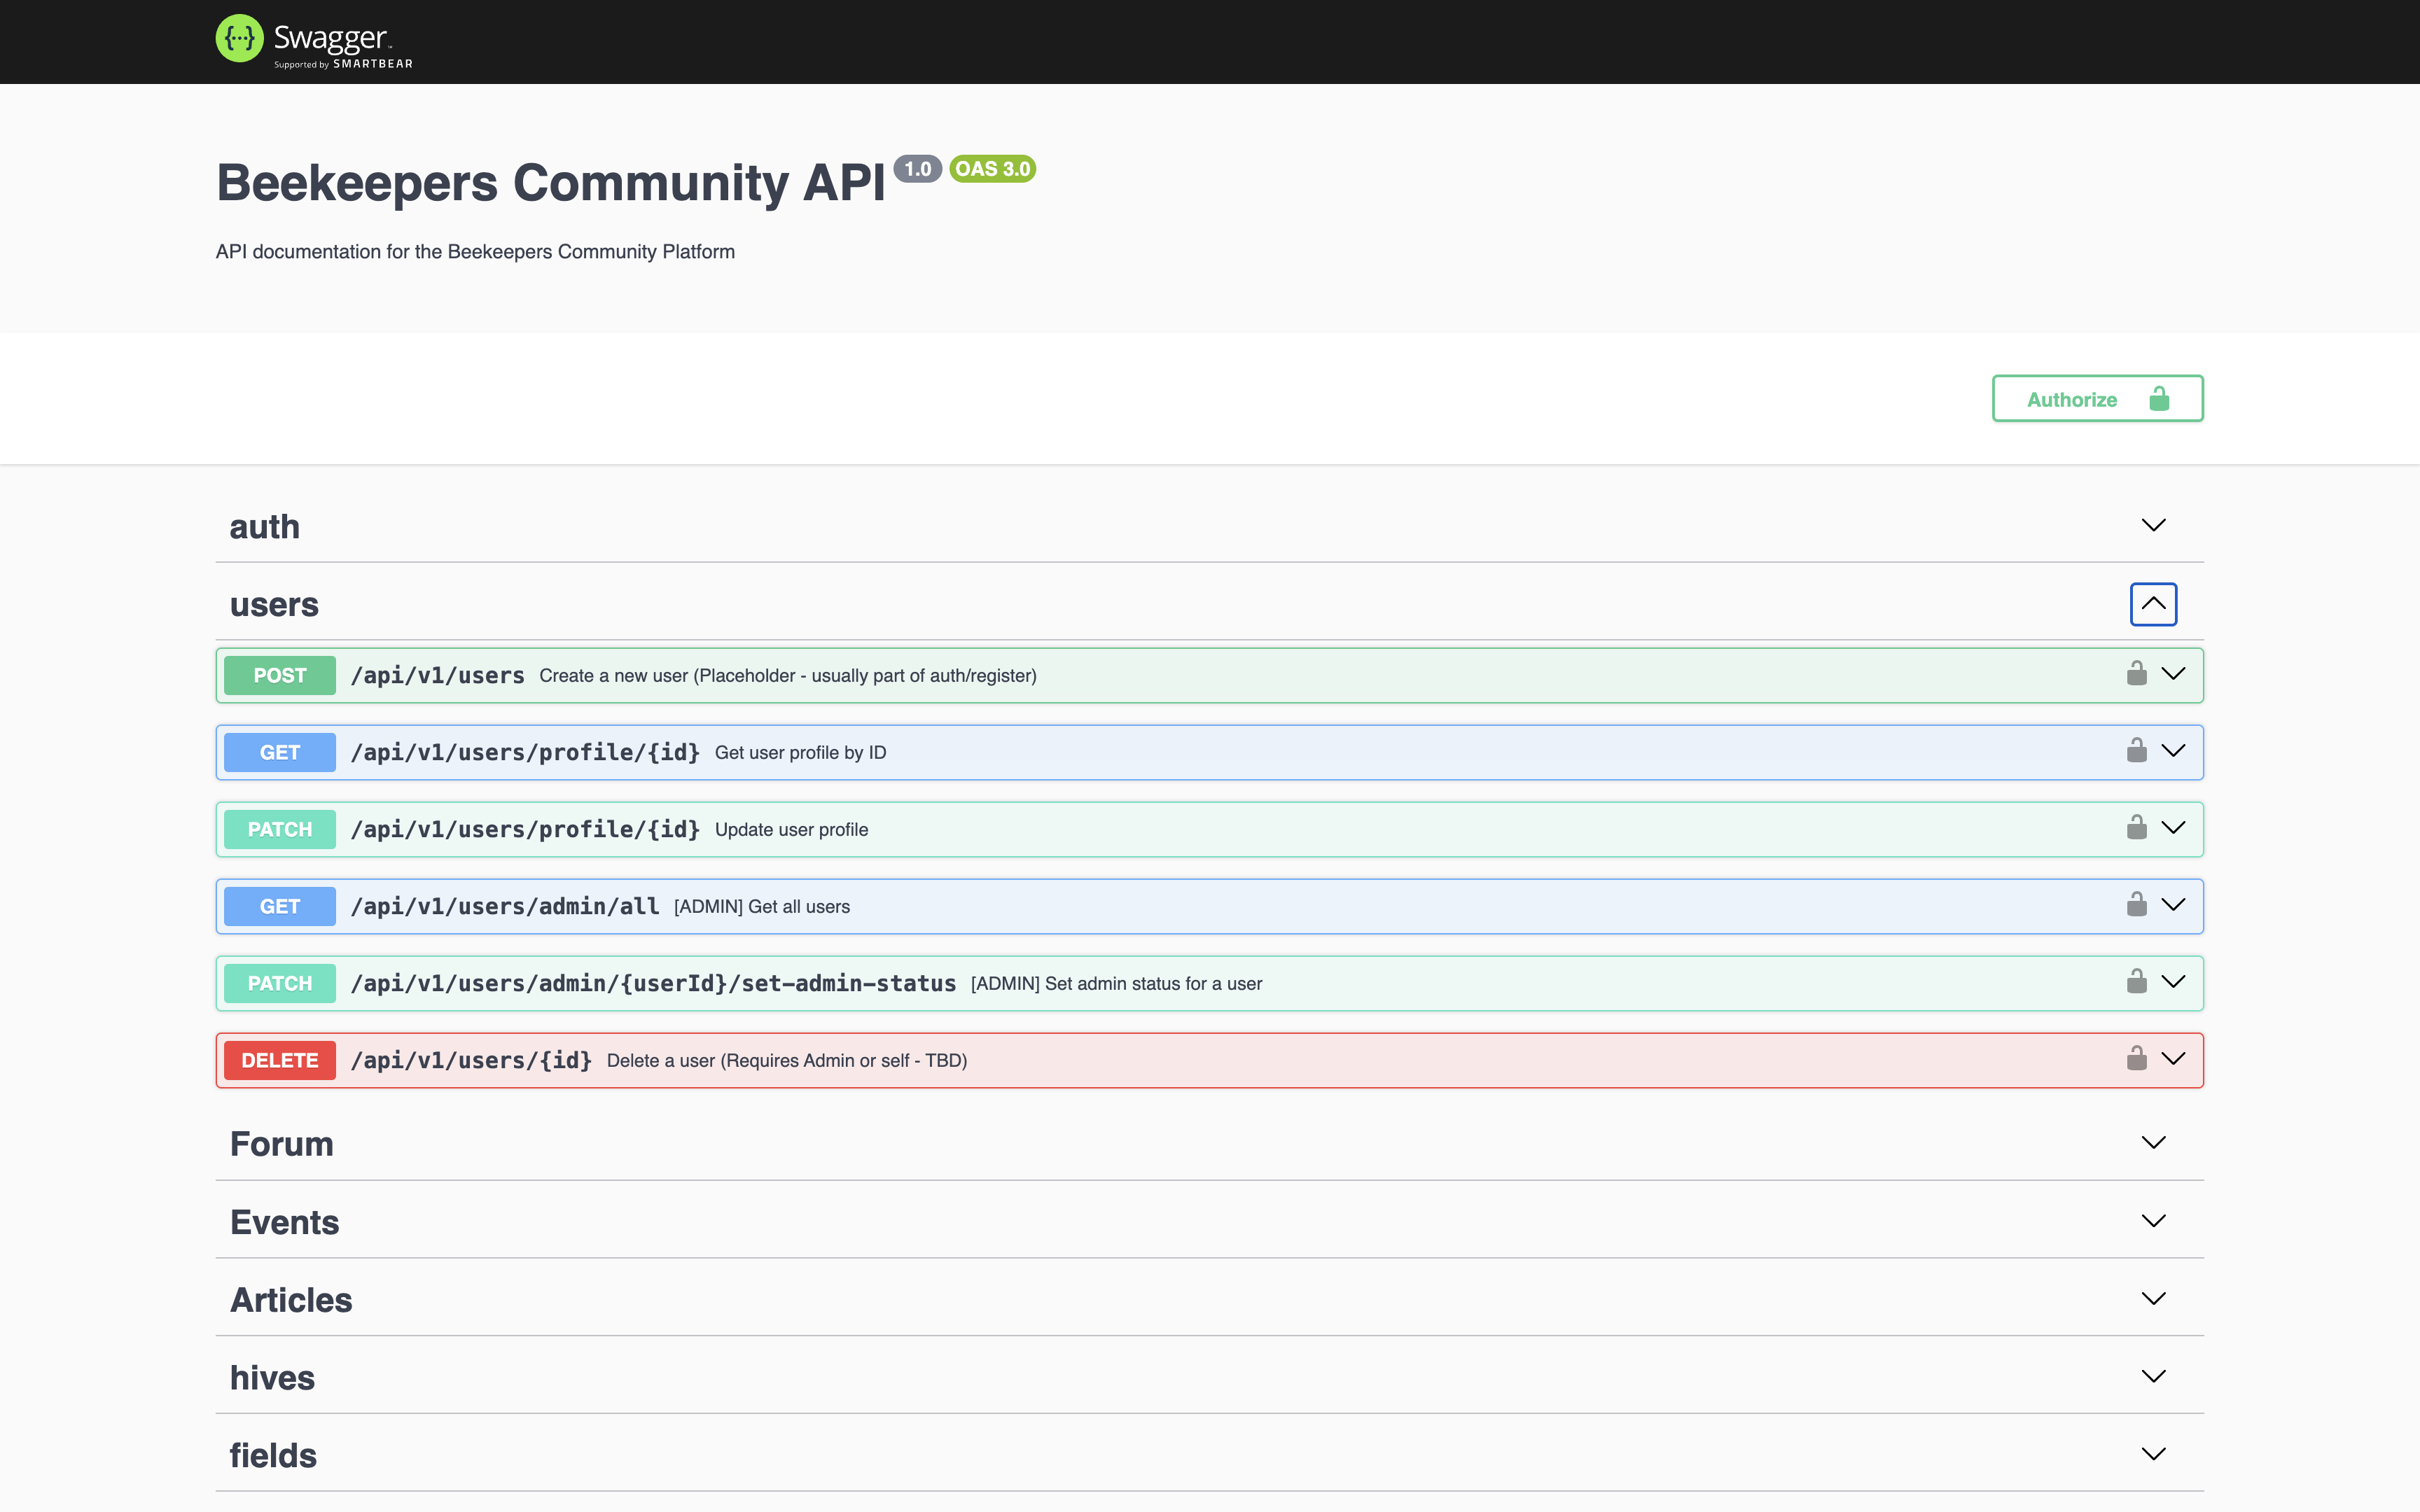
\includegraphics[width=0.9\textwidth]{practice_report/images/swagger.png}
  \caption{Головна сторінка документації API Beekeepers Community Platform у Swagger UI}
  \label{fig:swagger}
\end{figure}

% The User Manual chapter is now moved to the main body of the thesis.
% Old content removed from here.

% You can add other appendices here if needed, for example:
% \chapter{Додаткові діаграми}
% \label{app:other_diagrams}
% ... content ... 

\end{document} 